\documentclass[12pt,a4paper]{report}

\usepackage[utf8]{inputenc}
\usepackage{lmodern}
\usepackage[margin=1in]{geometry}
\usepackage{amsmath,amssymb,amsthm,mathtools}
\usepackage{booktabs}
\usepackage{tabularx}
\setlength{\emergencystretch}{2em}
\usepackage{graphicx}
\usepackage{float}
\usepackage{caption}
\usepackage{setspace}
\usepackage{fancyhdr}
\usepackage{listings}
\usepackage{xcolor}
\usepackage[colorlinks=true,linkcolor=black,citecolor=black,urlcolor=blue!40!black]{hyperref}

\setstretch{1.12}
\setlength{\headheight}{15pt}
\setlength{\parindent}{0pt}
\setlength{\parskip}{0.55em}
\captionsetup{font=small,labelfont=bf}

% ---------- Macros ----------
\newcommand{\R}{\mathbb{R}}
\newcommand{\norm}[1]{\lVert #1\rVert}
\newcommand{\T}{^{\top}}
\DeclareMathOperator{\rank}{rank}
\DeclareMathOperator{\Col}{Col}
\DeclareMathOperator{\diag}{diag}
\DeclareMathOperator{\tr}{tr}
% EDIT THIS LINE so that it matches the machine on which you re-run the code.
\newcommand{\runenv}{Python 3.13.16, NumPy 2.5.3, Matplotlib 3.11.2 (Darwin)}

% ---------- Theorem environments ----------
\theoremstyle{plain}
\newtheorem{theorem}{Theorem}[chapter]
\newtheorem{lemma}[theorem]{Lemma}
\newtheorem{proposition}[theorem]{Proposition}
\theoremstyle{definition}
\newtheorem{definition}[theorem]{Definition}
\theoremstyle{remark}
\newtheorem*{remark}{Remark}
\theoremstyle{definition}
\newtheorem{example}{Example}[chapter]

% ---------- Header / footer ----------
\pagestyle{fancy}
\fancyhf{}
\fancyhead[L]{\small SVD for Latent Semantic Analysis and Document Similarity}
\fancyhead[R]{\small MAC F211}
\fancyfoot[C]{\thepage}
\renewcommand{\headrulewidth}{0.4pt}
\fancypagestyle{plain}{\fancyhf{}\fancyfoot[C]{\thepage}\renewcommand{\headrulewidth}{0pt}}

% ---------- Code listings ----------
\lstset{
  language=Python,
  basicstyle=\ttfamily\footnotesize,
  keywordstyle=\bfseries,
  commentstyle=\itshape\color{black!60},
  stringstyle=\color{black!75},
  numbers=left, numberstyle=\tiny\color{black!55}, numbersep=6pt,
  breaklines=true, breakatwhitespace=false,
  frame=lines, framesep=4pt,
  showstringspaces=false, tabsize=4,
  literate={≈}{{$\approx$}}1,
  xleftmargin=1.6em
}

\begin{document}

% The cover page and the certificate sheet come from the official template and are
% printed and completed by hand, so this file begins at the Abstract. The counter below
% makes the Abstract page number ii, as it would be after the printed certificate page.
\pagenumbering{roman}
\setcounter{page}{2}

\chapter*{Abstract}
\addcontentsline{toc}{chapter}{Abstract}

The singular value decomposition (SVD) factorizes every real rectangular matrix into two orthogonal matrices and a diagonal matrix of non-negative singular values, and it gives the best low-rank approximation of a matrix in the Frobenius and spectral norms. In this report, the SVD is developed from the maximum principle for quadratic forms, following the course lectures, and is then specialized to a construction that needs only the eigen decomposition of the smaller of the two Gram matrices $A\T A$ and $AA\T$. The mathematical treatment covers the orthogonality of the singular vectors, the Eckart--Young theorem, the energy retained by a truncation, and the numerical price paid for working with a Gram matrix.

As an application, latent semantic analysis (LSA) compares plain-text documents using a custom TF-IDF matrix and reduced coordinates $\Sigma_kV_k\T$. Two five-document synthetic collections illustrate how rank truncation can strengthen same-topic similarities but also merge unrelated documents. A third experiment evaluates 250 real documents sampled from five categories of the 20 Newsgroups training subset. Its term--document matrix has 6,479 rows and numerical rank 250. Mean precision at five neighbours is 0.4976 for TF-IDF, compared with 0.2848, 0.4296, 0.4864 and 0.4928 for LSA ranks 5, 10, 20 and 50. Full-rank LSA recovers the baseline score. Thus no tested reduced rank improves mean precision on this sample. The evaluation excludes self-matches but searches the same collection used to fit TF-IDF and SVD; it is not a held-out query benchmark. The project demonstrates the construction, numerical verification and empirical limitations of Gram-matrix SVD for document similarity.

\bigskip
\noindent\textbf{Keywords:} singular value decomposition; Gram matrix; eigendecomposition; low-rank approximation; TF-IDF; cosine similarity; latent semantic analysis.

\clearpage
\tableofcontents
\clearpage
\pagenumbering{arabic}

\chapter{Mathematical Methods: Singular Value Decomposition}

\section{Literature Review}

The treatment of the SVD in this report follows the course lectures \cite{lectures}. There the singular values of a matrix $A$ are introduced through the eigenvalues of $A\T A$, the right singular vectors are the orthonormal eigenvectors of that matrix, the left singular vectors are obtained by applying $A$ to them, and the full decomposition $A=U\Sigma V\T$ is assembled from these pieces. The lectures also connect the singular values to the conditioning of a linear system, which is used in Section~\ref{sec:cond} below. The prescribed course textbooks \cite{lay,strang} cover the same material.

Three further sources shaped the remainder of the chapter. Eckart and Young \cite{eckartyoung} proved that truncating the SVD gives the best approximation of a given rank, and this result is the reason the SVD is useful for data compression and for latent semantic analysis. Golub and Van Loan \cite{golubvanloan} discuss the numerical computation of the SVD and explain why forming $A\T A$ explicitly loses accuracy for small singular values. Finally, Manning \cite{Manning}, Raghavan and Sch\"utze   present low-rank approximation of the term--document matrix in the context of information retrieval, which leads into the application of Chapter~2.

Some choices in my implementation go beyond the exact-arithmetic derivation given in the lectures: the use of the smaller Gram matrix, the scaling of the input, and the numerical rank threshold. These are explained and justified in Section~\ref{sec:numerics}. The symmetric eigenvalue problem itself is solved by NumPy's \texttt{numpy.linalg.eigh}, whose ordering and column conventions are documented in \cite{numpyeigh}. The program builds the SVD around this routine rather than implementing an eigensolver.

\section{Mathematical Method: Singular Value Decomposition}

\subsection{Why another decomposition?}

If a square matrix $A$ is diagonalisable, then $A=PDP^{-1}$, and the diagonal entries of $D$ describe how $A$ acts along its eigenvector directions. This is useful, but it has two limitations. The matrix must be square, and not every square matrix is diagonalisable. The QR factorisation $A=QR$ exists far more generally, but its second factor $R$ is triangular rather than diagonal, so it does not expose the action of $A$ as cleanly. The aim of the SVD is to find a diagonal-type factorisation that exists for \emph{every} $m\times n$ matrix.

The starting observation is geometric. For a symmetric matrix with $Av=\lambda v$ and $\norm{v}=1$ we have $\norm{Av}=|\lambda|$, so an eigenvector belonging to an eigenvalue of largest magnitude is a direction of greatest stretching. For a rectangular matrix $A:\R^n\to\R^m$ the equation $Ax=\lambda x$ does not even make sense, but the geometric question still does: among all unit vectors $x$, for which $x$ is $\norm{Ax}$ largest? The answer will come from a symmetric matrix that can always be built from $A$.

\subsection{The maximum principle for quadratic forms}

\begin{theorem}[Maximum principle]\label{thm:maxprinciple}
Let $G$ be a real symmetric $n\times n$ matrix with eigenvalues $\lambda_1\ge\lambda_2\ge\dots\ge\lambda_n$ and corresponding orthonormal eigenvectors $v_1,\dots,v_n$. Then
\[
\max_{\norm{x}=1} x\T G x=\lambda_1,
\qquad
\min_{\norm{x}=1} x\T G x=\lambda_n,
\]
and the maximum is attained at $x=v_1$. More generally, for $k\ge 2$,
\[
\max\{\,x\T Gx:\ \norm{x}=1,\ x\perp v_1,\dots,v_{k-1}\,\}=\lambda_k ,
\]
attained at $x=v_k$.
\end{theorem}

\begin{proof}
By the spectral theorem $G=Q\Lambda Q\T$ with $Q=[v_1\ \cdots\ v_n]$ orthogonal. Put $y=Q\T x$, so that $\norm{y}=\norm{x}=1$ and $x\T Gx=y\T\Lambda y=\sum_{i}\lambda_i y_i^2$. Since the weights $y_i^2$ are non-negative and sum to one, this is a weighted average of the eigenvalues. It is therefore at most $\lambda_1$, with equality when $y=e_1$, that is, $x=v_1$. The minimum is handled in the same way. If $x\perp v_1,\dots,v_{k-1}$ then $y_1=\dots=y_{k-1}=0$, and the same argument applied to $\sum_{i\ge k}\lambda_iy_i^2$ gives the bound $\lambda_k$, attained at $y=e_k$.
\end{proof}

\subsection{Singular values and singular vectors}

Let $A$ be an $m\times n$ real matrix. For every $x\in\R^n$,
\begin{equation}\label{eq:normsq}
\norm{Ax}^2=(Ax)\T(Ax)=x\T(A\T A)x .
\end{equation}
The matrix $A\T A$ is symmetric, and equation~\eqref{eq:normsq} shows that $x\T(A\T A)x=\norm{Ax}^2\ge 0$, so it is positive semidefinite and all its eigenvalues are non-negative. Choose an orthonormal eigenbasis $v_1,\dots,v_n$ of $\R^n$ with
\[
A\T A\,v_i=\lambda_i v_i,\qquad \lambda_1\ge\lambda_2\ge\dots\ge\lambda_n\ge 0 .
\]
Then $\norm{Av_i}^2=v_i\T A\T Av_i=\lambda_i$.

\begin{definition}[Singular values and singular vectors]
The \emph{singular values} of $A$ are $\sigma_i=\sqrt{\lambda_i}=\norm{Av_i}$, arranged so that $\sigma_1\ge\sigma_2\ge\dots\ge\sigma_n\ge 0$. The vectors $v_i$ are the \emph{right singular vectors} of $A$.
\end{definition}

Theorem~\ref{thm:maxprinciple} applied to $G=A\T A$ gives the variational meaning of the singular values:
\[
\sigma_1=\max_{\norm{x}=1}\norm{Ax}\ \ (\text{attained at }v_1),\qquad
\sigma_k=\max_{\substack{\norm{x}=1\\ x\perp v_1,\dots,v_{k-1}}}\norm{Ax}\ \ (\text{attained at }v_k).
\]
In words, $v_1,v_2,\dots$ are successive orthogonal input directions of greatest remaining stretch, and $\sigma_i$ is the amount of stretching along $v_i$. In particular $\sigma_1=\norm{A}_2$, the spectral norm.

\subsection{Output directions, rank and the column space}

For $i\ne j$,
\[
(Av_i)\T(Av_j)=v_i\T A\T A v_j=\lambda_j\,v_i\T v_j=0 ,
\]
so the vectors $Av_1,\dots,Av_n$ are mutually orthogonal. Those with $\sigma_i=0$ have length zero and therefore equal the zero vector.

\begin{theorem}[Column space and rank]\label{thm:colspace}
Suppose $A$ has exactly $r$ nonzero singular values, so that $\sigma_1\ge\dots\ge\sigma_r>0=\sigma_{r+1}=\dots=\sigma_n$. Then $\{Av_1,\dots,Av_r\}$ is an orthogonal basis of $\Col A$, and $\rank A=r$.
\end{theorem}

\begin{proof}
Any $y\in\Col A$ has the form $y=Ax$ with $x=\sum_{i=1}^n c_iv_i$. Because $Av_i=0$ for $i>r$, we get $y=\sum_{i=1}^r c_iAv_i$, so $Av_1,\dots,Av_r$ span $\Col A$. They are nonzero and mutually orthogonal, hence linearly independent, so they form a basis and $\dim\Col A=r$.
\end{proof}

For each $i\le r$ define the \emph{left singular vector}
\[
u_i=\frac{Av_i}{\sigma_i}.
\]
Then $\norm{u_i}=1$ and $u_i\T u_j=0$ for $i\ne j$, so $u_1,\dots,u_r$ are orthonormal, and
\begin{equation}\label{eq:pairs}
Av_i=\sigma_iu_i,\qquad A\T u_i=\frac{A\T Av_i}{\sigma_i}=\frac{\lambda_iv_i}{\sigma_i}=\sigma_iv_i .
\end{equation}
Geometrically, $v_i$ is a special input direction, $\sigma_i$ is the stretching factor, and $u_i$ is the direction in which the image lies. Moreover, by Theorem~\ref{thm:colspace} the vectors $u_1,\dots,u_r$ form an orthonormal basis of $\Col A$.

\subsection{The singular value decomposition theorem}

For an $m\times n$ matrix of rank $r$ let $D=\diag(\sigma_1,\dots,\sigma_r)$ and let $\Sigma\in\R^{m\times n}$ be the matrix
\[
\Sigma=\begin{bmatrix} D&0\\0&0\end{bmatrix}.
\]
It has the same size as $A$, and its only nonzero entries are the singular values on the main diagonal.

\begin{theorem}[Singular value decomposition]\label{thm:svd}
Let $A$ be a real $m\times n$ matrix of rank $r$. Then there are orthogonal matrices $U\in\R^{m\times m}$ and $V\in\R^{n\times n}$ such that
\[
A=U\Sigma V\T .
\]
The positive diagonal entries of $\Sigma$ are $\sigma_1\ge\dots\ge\sigma_r>0$. The columns of $U$ and $V$ are the left and right singular vectors.
\end{theorem}

\begin{proof}
Take $V=[v_1\ \cdots\ v_n]$, whose columns are the orthonormal eigenvectors of $A\T A$ chosen above, so $V\T V=I_n$. Take $u_1,\dots,u_r$ as defined above and extend them to an orthonormal basis $u_1,\dots,u_m$ of $\R^m$ (possible because they are orthonormal). Put $U=[u_1\ \cdots\ u_m]$, so $U\T U=I_m$. Now
\[
U\Sigma=[\sigma_1u_1\ \cdots\ \sigma_ru_r\ 0\ \cdots\ 0]=[Av_1\ \cdots\ Av_r\ Av_{r+1}\ \cdots\ Av_n]=AV,
\]
where we used $\sigma_iu_i=Av_i$ for $i\le r$ and $Av_i=0$ for $i>r$. Since $V$ is orthogonal, multiplying $U\Sigma=AV$ on the right by $V\T$ gives $A=U\Sigma V\T$.
\end{proof}

The proof is also a recipe. \emph{Step 1:} compute $A\T A$ and an orthonormal eigenbasis, ordered by decreasing eigenvalue, and set $\sigma_i=\sqrt{\lambda_i}$. \emph{Step 2:} form $\Sigma$. \emph{Step 3:} set $u_i=Av_i/\sigma_i$ for $i\le r$ and, if $r<m$, complete to an orthonormal basis of $\R^m$.

\subsection{Compact form}

The columns $u_{r+1},\dots,u_m$ and $v_{r+1},\dots,v_n$ multiply zero blocks of $\Sigma$, so they do not contribute to the product. Dropping them gives the \emph{compact SVD}
\begin{equation}\label{eq:compact}
A=U_r\Sigma_rV_r\T=\sum_{i=1}^r\sigma_i\,u_iv_i\T,\qquad \Sigma_r=\diag(\sigma_1,\dots,\sigma_r),
\end{equation}
where $U_r\in\R^{m\times r}$ and $V_r\in\R^{n\times r}$ have orthonormal columns, so $U_r\T U_r=V_r\T V_r=I_r$. Note that $U_rU_r\T\ne I_m$ in general; it is the orthogonal projector onto $\Col A$. This compact form is what the program returns and the text application needs nothing more.

\subsection{Gram matrices and the choice of the smaller one}\label{sec:gram}

For a matrix $B$ with columns $b_1,\dots,b_n$, the \emph{Gram matrix} is $G=B\T B$ with entries $G_{ij}=b_i\T b_j$. Its diagonal entries are squared lengths and its off-diagonal entries are dot products; they are cosines only if the columns have been normalised. The matrix $BB\T$ is the Gram matrix of the rows of $B$. Both matrices are symmetric and positive semidefinite, since $x\T B\T Bx=\norm{Bx}^2$ and $y\T BB\T y=\norm{B\T y}^2$. For $B$ with columns $(1,1,0)\T$ and $(1,0,1)\T$,
\[
B=\begin{bmatrix}1&1\\1&0\\0&1\end{bmatrix},\qquad B\T B=\begin{bmatrix}2&1\\1&2\end{bmatrix}.
\]
For a term--document matrix, $B\T B$ stores dot products between documents, and $BB\T$ stores dot products between the occurrence patterns of terms.

The construction in Theorem~\ref{thm:svd} uses the right Gram matrix $A\T A$, which is $n\times n$. When $A$ is wide ($m<n$) it is cheaper to work with the left Gram matrix $AA\T$, which is $m\times m$. The next lemma shows that nothing is lost.

\begin{lemma}\label{lem:gram}
The positive eigenvalues of $A\T A$ and $AA\T$ coincide, with the same multiplicities. If $AA\T u_i=\lambda_iu_i$ with $\lambda_i=\sigma_i^2>0$ and $u_1,\ldots,u_r$ form an orthonormal basis of the direct sum of all positive-eigenvalue eigenspaces of $AA\T$, then the vectors $v_i=A\T u_i/\sigma_i$ are orthonormal, satisfy $A\T Av_i=\lambda_iv_i$, and
\[
A=\sum_{i}\sigma_i u_iv_i\T .
\]
\end{lemma}

\begin{proof}
Let $A\T Av=\lambda v$ with $\lambda>0$. Then $Av\ne0$, because $\norm{Av}^2=\lambda\norm{v}^2>0$, and $AA\T(Av)=A(A\T Av)=\lambda\,Av$. Hence $A$ maps the $\lambda$-eigenspace of $A\T A$ into that of $AA\T$. The same argument with $A\T$ gives a map in the other direction, and the two maps are inverse to each other up to the factor $\lambda$. So the eigenspaces have equal dimension.

Now let $u_i$ be as in the statement. Then
\[
v_i\T v_j=\frac{u_i\T AA\T u_j}{\sigma_i\sigma_j}=\frac{\lambda_j}{\sigma_i\sigma_j}u_i\T u_j=\delta_{ij},
\qquad
A\T Av_i=\frac{A\T(AA\T u_i)}{\sigma_i}=\lambda_i v_i,
\]
and $Av_i=AA\T u_i/\sigma_i=\sigma_iu_i$. For the reconstruction, the retained $u_i$ with $\lambda_i>0$ span $\Col A$, so $U_rU_r\T A=A$. Also $A\T u_i=\sigma_iv_i$ gives $\sigma_iv_i\T=u_i\T A$, that is, $\Sigma_rV_r\T=U_r\T A$. Therefore $U_r\Sigma_rV_r\T=U_rU_r\T A=A$.
\end{proof}

The zero eigenvalues of the two Gram matrices need not agree: there are $n-r$ of them for $A\T A$ and $m-r$ for $AA\T$. The labels are never interchanged: eigenvectors of $AA\T$ are left singular vectors, and eigenvectors of $A\T A$ are right singular vectors. For a dense matrix, forming the smaller Gram matrix costs $O(mn\min(m,n))$ operations and a dense symmetric eigendecomposition of it costs $O(\min(m,n)^3)$. This reduces the size of the eigenproblem; it does not make the method sparse or iterative.

\subsection{Non-uniqueness}\label{sec:nonunique}

The singular values are unique, but the singular vectors are not. Replacing a pair $(u_i,v_i)$ by $(-u_i,-v_i)$ leaves $A=\sum\sigma_iu_iv_i\T$ unchanged. If a singular value is repeated, any orthogonal rotation of the corresponding block of right singular vectors, together with the matching rotation of the left ones, gives another valid SVD. For example, $(e_1,e_2)$ and $\bigl((e_1+e_2)/\sqrt2,\,(e_1-e_2)/\sqrt2\bigr)$ are both orthonormal bases of the eigenspace belonging to the double eigenvalue $2$ of $\diag(2,2,5)$. For this reason the program fixes a sign convention (the largest entry of each $u_i$ in absolute value is made positive), but it cannot remove the freedom caused by repeated singular values. Checks on a computed SVD should therefore compare invariant quantities, namely the singular values, the reconstruction, and orthogonality, rather than individual vector entries.

\subsection{Low-rank approximation}\label{sec:eckartyoung}

Keeping only the first $k<r$ terms of~\eqref{eq:compact} gives the \emph{truncated SVD}
\[
A_k=U_k\Sigma_kV_k\T=\sum_{i=1}^k\sigma_iu_iv_i\T,
\]
a matrix of rank $k$. Unlike the compact SVD, it is a genuine approximation of $A$. Two facts are needed: $\norm{A}_F^2=\tr(A\T A)=\sum_i\lambda_i=\sum_i\sigma_i^2$, and the matrices $u_iv_i\T$ are orthonormal with respect to the Frobenius inner product $\langle X,Y\rangle=\tr(X\T Y)$.

\begin{theorem}[Eckart--Young]\label{thm:ey}
For $0\le k<r$,
\[
\norm{A-A_k}_2=\sigma_{k+1},\qquad \norm{A-A_k}_F^2=\sum_{i=k+1}^r\sigma_i^2 ,
\]
and for every matrix $X$ with $\rank X\le k$,
\[
\norm{A-X}_2\ge\sigma_{k+1},\qquad \norm{A-X}_F^2\ge\sum_{i=k+1}^r\sigma_i^2 .
\]
So $A_k$ is a best rank-$k$ approximation in both norms.
\end{theorem}

\begin{proof}
\emph{The errors of $A_k$.} We have $A-A_k=\sum_{i>k}\sigma_iu_iv_i\T$, which is an SVD with largest singular value $\sigma_{k+1}$ and squared Frobenius norm $\sum_{i>k}\sigma_i^2$.

\emph{Spectral optimality.} Let $\rank X\le k$. Its null space has dimension at least $n-k$, while $W=\operatorname{span}\{v_1,\dots,v_{k+1}\}$ has dimension $k+1$. Since $(n-k)+(k+1)>n$, the two subspaces share a unit vector $x$. For this $x$, $Xx=0$ and $x=\sum_{i\le k+1}c_iv_i$ with $\sum c_i^2=1$, so
\[
\norm{(A-X)x}^2=\norm{Ax}^2=\sum_{i\le k+1}\sigma_i^2c_i^2\ge\sigma_{k+1}^2 .
\]
Hence $\norm{A-X}_2\ge\sigma_{k+1}$.

\emph{Frobenius optimality.} Let $P$ be the orthogonal projector onto $\Col X$, which has dimension at most $k$. Then $(I-P)X=0$, and since $I-P$ cannot increase the Frobenius norm,
\[
\norm{A-X}_F^2\ge\norm{(I-P)(A-X)}_F^2=\norm{(I-P)A}_F^2=\norm{A}_F^2-\norm{PA}_F^2,
\]
where the last step is Pythagoras applied column by column. Because the $v_i$ are orthonormal, $\norm{PA}_F^2=\sum_{i=1}^r\sigma_i^2\,\norm{Pu_i}^2$. The weights $w_i=\norm{Pu_i}^2$ lie in $[0,1]$, and $\sum_iw_i\le\norm{P}_F^2=\rank P\le k$ since the $u_i$ are orthonormal. Because $\sigma_1\ge\sigma_2\ge\cdots$, the sum $\sum_i\sigma_i^2w_i$ is largest when the weight is concentrated on the first $k$ indices, so it is at most $\sum_{i\le k}\sigma_i^2$. Therefore $\norm{A-X}_F^2\ge\sum_{i=1}^r\sigma_i^2-\sum_{i\le k}\sigma_i^2=\sum_{i>k}\sigma_i^2$.
\end{proof}

When singular values at the cut-off are repeated, for example $\sigma_k=\sigma_{k+1}$, the best rank-$k$ approximation is not unique.

\subsection{Energy and conditioning}\label{sec:cond}

Define the \emph{retained energy}
\[
E(k)=\frac{\sum_{i=1}^k\sigma_i^2}{\sum_{i=1}^r\sigma_i^2}.
\]
By Theorem~\ref{thm:ey} the relative Frobenius error of the truncation is
\begin{equation}\label{eq:relerr}
\frac{\norm{A-A_k}_F}{\norm{A}_F}=\sqrt{1-E(k)} .
\end{equation}
A target of 90\% energy therefore permits a relative error as large as $\sqrt{0.1}\approx31.6\%$, not 10\%. This distinction matters when the energy is used to pick $k$ in Chapter~2.

The lectures relate the singular values to conditioning. For an invertible $n\times n$ matrix, $\sigma_1=\max_{\norm{x}=1}\norm{Ax}$ and $\sigma_n=\min_{\norm{x}=1}\norm{Ax}$, so the 2-norm condition number is
\[
\kappa_2(A)=\frac{\sigma_1}{\sigma_n}.
\]
A very small $\sigma_n$ means that some input direction is almost collapsed by $A$, and a large ratio signals strong sensitivity of $Ax=b$ to perturbations. For a rectangular matrix of full column rank the same ratio $\sigma_1/\sigma_r$ is used, and
\begin{equation}\label{eq:kappasq}
\kappa_2(A\T A)=\left(\frac{\sigma_1}{\sigma_r}\right)^2 ,
\end{equation}
because the eigenvalues of $A\T A$ are $\sigma_i^2$. A rank-deficient Gram matrix is singular, so ratios of its positive eigenvalues describe only its action on the nonzero subspace.

For a truncation I report $\kappa_{\mathrm{ret}}(k)=\sigma_1/\sigma_k$, the condition number of the retained block $\Sigma_k$. This number must be read with care. It is not an ordinary condition number of the rank-$k$ matrix $A_k$, which is singular when $k<\min(m,n)$, and it equals one for $k=1$ no matter how much information the truncation destroys. Numerical stability and usefulness for retrieval are different questions.

\subsection{Numerical considerations and the algorithm}\label{sec:numerics}

Equation~\eqref{eq:kappasq} has a practical consequence. The eigenvalue routine works on the computed Gram matrix, whose rounding errors are of size about $\varepsilon\sigma_1^2$ in absolute terms, where $\varepsilon\approx2.2\times10^{-16}$ is the double-precision machine epsilon. An eigenvalue $\lambda_i=\sigma_i^2$ perturbed by $\delta\lambda$ changes $\sigma_i=\sqrt{\lambda_i}$ by roughly $\delta\lambda/(2\sigma_i)$, so the relative error in $\sigma_i$ is of order $\varepsilon(\sigma_1/\sigma_i)^2$. Small singular values are therefore resolved much less accurately than by an SVD routine that works on $A$ directly, such as the LAPACK routine behind NumPy's SVD function \cite{numpysvd,golubvanloan}. The reported reconstruction and full-rank cosine checks are close to floating-point precision for the collections studied here. This empirical observation does not remove the accuracy limitation for ill-conditioned matrices.

The program in Appendix~A proceeds as follows.
\begin{enumerate}
\item Reject complex, non-finite, empty or non-two-dimensional input, and convert to double precision.
\item Let $c=\max_{ij}|A_{ij}|$. If $c=0$, return empty factors of shapes $(m,0)$, $(0,0)$ and $(0,n)$, since the zero matrix has rank zero. Otherwise set $B=A/c$. This keeps the entries of the Gram matrix at a safe magnitude; it does not improve the condition number.
\item Form $G=B\T B$ if $m\ge n$ and $G=BB\T$ otherwise, and compute its eigenpairs with \texttt{numpy.linalg.eigh}. Sort eigenvalues and eigenvector columns together in decreasing order.
\item Set the tolerance $\tau=10\,\varepsilon\max(m,n)\,\lambda_{\max}$. Raise an error if some eigenvalue is below $-\tau$ (a significantly negative eigenvalue of a positive semidefinite matrix signals a failure), and keep only the eigenvalues strictly greater than $\tau$.
\item Take square roots of the retained eigenvalues to get the scaled singular values, and recover the other factor by $u_i=Bv_i/s_i$ or $v_i=B\T u_i/s_i$ (Lemma~\ref{lem:gram}).
\item Apply the paired sign convention, restore the scale $\sigma_i=c\,s_i$, check that the restored values are finite, and return $U_r$, $\diag(\sigma_i)$ and $V_r\T$.
\end{enumerate}
Division is carried out only by singular values that passed the tolerance. The factor ten in $\tau$ is a heuristic and not an optimal universal error bound. Because a singular value is the square root of an eigenvalue, the threshold corresponds to discarding singular values with $\sigma_i/\sigma_1$ below about $\sqrt{10\,\varepsilon\max(m,n)}$; for $m=125$ this is roughly $5\times10^{-7}$. Dividing by a small retained $\sigma_i$ can amplify errors, so both factors are checked for orthogonality in Chapter~2.

\subsection{Why the SVD rather than QR, diagonalisation or the Jordan form?}

QR gives an orthonormal basis and a triangular factor and is the tool of choice for least squares, but it does not order orthogonal components by their contribution to the best low-rank approximation. Diagonalisation and the Jordan form describe similarity transformations of square matrices; a diagonalisation need not exist and the change of basis need not be orthogonal. The SVD exists for every real rectangular matrix, has orthonormal factors, and directly supplies the optimal rank-$k$ approximation of Theorem~\ref{thm:ey}, which is exactly what the application requires.

\section{Examples of the Mathematical Method}

\begin{example}[The class example, via $A\T A$]\label{ex:class}
Let
\[
A=\begin{bmatrix}4&11&14\\8&7&-2\end{bmatrix},\qquad
A\T A=\begin{bmatrix}80&100&40\\100&170&140\\40&140&200\end{bmatrix}.
\]
The eigenvalues of $A\T A$ are $\lambda_1=360$, $\lambda_2=90$ and $\lambda_3=0$ (their sum is $450=\tr A\T A$), with orthonormal eigenvectors
\[
v_1=\tfrac13\begin{bmatrix}1\\2\\2\end{bmatrix},\quad
v_2=\tfrac13\begin{bmatrix}-2\\-1\\2\end{bmatrix},\quad
v_3=\tfrac13\begin{bmatrix}2\\-2\\1\end{bmatrix}.
\]
Hence $\sigma_1=\sqrt{360}=6\sqrt{10}$, $\sigma_2=\sqrt{90}=3\sqrt{10}$ and $\sigma_3=0$, so $\rank A=2$. Next,
\[
Av_1=\begin{bmatrix}18\\6\end{bmatrix},\quad Av_2=\begin{bmatrix}3\\-9\end{bmatrix},\quad Av_3=\begin{bmatrix}0\\0\end{bmatrix},
\qquad
u_1=\frac{1}{\sqrt{10}}\begin{bmatrix}3\\1\end{bmatrix},\quad u_2=\frac1{\sqrt{10}}\begin{bmatrix}1\\-3\end{bmatrix}.
\]
These are orthonormal ($3\cdot1+1\cdot(-3)=0$), so
\[
U=\frac1{\sqrt{10}}\begin{bmatrix}3&1\\1&-3\end{bmatrix},\quad
\Sigma=\begin{bmatrix}6\sqrt{10}&0&0\\0&3\sqrt{10}&0\end{bmatrix},\quad
V=\frac13\begin{bmatrix}1&-2&2\\2&-1&-2\\2&2&1\end{bmatrix}.
\]
To confirm $A=U\Sigma V\T$, use $A=\sigma_1u_1v_1\T+\sigma_2u_2v_2\T=\binom{18}{6}v_1\T+\binom{3}{-9}v_2\T$. The first row is
$18\cdot\tfrac13(1,2,2)+3\cdot\tfrac13(-2,-1,2)=(6,12,12)+(-2,-1,2)=(4,11,14)$,
and the second row is
$6\cdot\tfrac13(1,2,2)-9\cdot\tfrac13(-2,-1,2)=(2,4,4)+(6,3,-6)=(8,7,-2)$.

The rank-one truncation is $A_1=\binom{18}{6}v_1\T=\begin{bmatrix}6&12&12\\2&4&4\end{bmatrix}$. Its error matrix $A-A_1=\begin{bmatrix}-2&-1&2\\6&3&-6\end{bmatrix}$ has squared Frobenius norm $4+1+4+36+9+36=90=\sigma_2^2$, as Theorem~\ref{thm:ey} predicts, and $E(1)=360/450=0.8$.
\end{example}

\begin{example}[The same matrix via $AA\T$]\label{ex:left}
For the $2\times3$ matrix of Example~\ref{ex:class} the left Gram matrix is smaller:
\[
AA\T=\begin{bmatrix}333&81\\81&117\end{bmatrix},\qquad \lambda^2-450\lambda+32400=(\lambda-360)(\lambda-90)=0 .
\]
The eigenvalues are the same positive ones as before, and the extra zero eigenvalue of $A\T A$ is absent. Unit eigenvectors are $u_1=(3,1)\T/\sqrt{10}$ and $u_2=(1,-3)\T/\sqrt{10}$; one checks, for instance, $AA\T(1,-3)\T=(90,-270)\T=90\,(1,-3)\T$. Lemma~\ref{lem:gram} recovers the right singular vectors:
\[
v_1=\frac{A\T u_1}{\sigma_1}=\frac{(20,40,40)\T}{\sqrt{10}\cdot6\sqrt{10}}=\tfrac13\begin{bmatrix}1\\2\\2\end{bmatrix},\qquad
v_2=\frac{A\T u_2}{\sigma_2}=\frac{(-20,-10,20)\T}{\sqrt{10}\cdot3\sqrt{10}}=\tfrac13\begin{bmatrix}-2\\-1\\2\end{bmatrix}.
\]
These agree with Example~\ref{ex:class}, so the $2\times2$ eigenproblem produced the same compact SVD without solving the $3\times3$ one.
\end{example}

\begin{example}[A tall matrix and its best rank-one approximation]\label{ex:tall}
Let
\[
A=\begin{bmatrix}1&1\\1&0\\0&1\end{bmatrix},\qquad A\T A=\begin{bmatrix}2&1\\1&2\end{bmatrix}.
\]
The characteristic equation $(2-\lambda)^2-1=0$ gives $\lambda_1=3$ and $\lambda_2=1$, with $v_1=\tfrac1{\sqrt2}(1,1)\T$ and $v_2=\tfrac1{\sqrt2}(1,-1)\T$. Thus $\sigma_1=\sqrt3$, $\sigma_2=1$, and
\[
u_1=\frac{Av_1}{\sqrt3}=\frac1{\sqrt6}\begin{bmatrix}2\\1\\1\end{bmatrix},\qquad
u_2=Av_2=\frac1{\sqrt2}\begin{bmatrix}0\\1\\-1\end{bmatrix}.
\]
The rank-one approximation is
\[
A_1=\sigma_1u_1v_1\T=\frac{\sqrt3}{\sqrt{12}}\begin{bmatrix}2\\1\\1\end{bmatrix}\begin{bmatrix}1&1\end{bmatrix}=\begin{bmatrix}1&1\\\tfrac12&\tfrac12\\\tfrac12&\tfrac12\end{bmatrix},
\]
and $A-A_1$ has four entries of magnitude $\tfrac12$, so $\norm{A-A_1}_F^2=4\cdot\tfrac14=1=\sigma_2^2$. Since $\norm{A}_F^2=4$, the retained energy is $E(1)=3/4$ and the relative error is $\sqrt{1-3/4}=1/2$, in agreement with~\eqref{eq:relerr}.
\end{example}

\begin{example}[A rank-deficient matrix]\label{ex:rankdef}
Let
\[
A=\begin{bmatrix}1&1\\2&2\\2&2\end{bmatrix},\qquad A\T A=\begin{bmatrix}9&9\\9&9\end{bmatrix}.
\]
The characteristic polynomial is $\lambda(\lambda-18)$, so $\lambda_1=18$, $\lambda_2=0$, and $\rank A=1$. The unit eigenvector for $18$ is $v_1=\tfrac1{\sqrt2}(1,1)\T$, so $\sigma_1=3\sqrt2$ and
\[
u_1=\frac{Av_1}{3\sqrt2}=\tfrac13\begin{bmatrix}1\\2\\2\end{bmatrix}.
\]
The compact SVD $A=u_1\sigma_1v_1\T=\tfrac13(1,2,2)\T\,[3\sqrt2]\,\tfrac1{\sqrt2}(1,1)$ already reproduces $A$ exactly. The second right singular vector $v_2=\tfrac1{\sqrt2}(1,-1)\T$ lies in the null space of $A$, and dividing $Av_2=0$ by $\sigma_2=0$ would be meaningless. A full SVD needs the missing left vectors only to complete a basis of $\R^3$; any orthonormal completion works, for instance $\tfrac13(2,1,-2)\T$ and $\tfrac13(2,-2,1)\T$, both orthogonal to $u_1$ and to each other. They multiply zero rows of $\Sigma$ and do not affect the product.
\end{example}

\chapter{An Application of SVD: Document Similarity}

\section{Literature Review: Introduction to the Problem/Application}

Collections of reports, emails, support tickets or notes often contain documents that are about the same thing but are written with different words. A search system, a clustering routine or a duplicate detector has to decide how close two documents are. A count-based vector representation turns the question into a numerical one: every distinct word becomes a coordinate, and a document becomes a vector of word counts. This ignores word order, but it is simple and it works surprisingly well as a first approximation  .

Raw counts have two well-known weaknesses. Common words dominate the counts although they say little about the topic, and two documents on the same topic may share few words because they choose different vocabulary. The first is usually addressed by reweighting terms according to how many documents contain them (the TF-IDF weighting), and the second is the motivation for latent semantic analysis (LSA), introduced by Deerwester and co-authors \cite{deerwester}. LSA replaces the high-dimensional word-count representation by a low-rank one obtained from the SVD of the term--document matrix  .

For the representation of text as a matrix I started from an introductory article on the term--document matrix (TDM) and the document--term matrix (DTM) \cite{girdher}. In this report terms index the rows and documents index the columns, so the matrix is the TDM; its transpose is the DTM. The application compares the plain-text documents of one collection with each other. No pretrained embeddings are used: all representations are computed from the collection itself. The documents used are five short synthetic passages written for illustration (see Section~\ref{sec:dataset}); they are not an independently collected benchmark.

\section{Where and Why the Method is Used}

The SVD enters after the TF-IDF weighting has produced a matrix $A\in\R^{m\times N}$ with one row per term and one column per document. The compact SVD $A=U_r\Sigma_rV_r\T$ of Chapter~1 sorts the orthogonal directions of this matrix by singular value. The columns of $U_r$ are directions in term space, each a weighted combination of words that tend to occur together; the rows of $V_r\T$ record how strongly each document uses those directions.

Truncating after $k$ terms keeps the $k$ strongest of these shared patterns and discards the rest. By the Eckart--Young theorem (Theorem~\ref{thm:ey}) the truncated matrix $A_k$ is the rank-$k$ matrix closest to $A$ in the Frobenius norm, so no other rank-$k$ reduction preserves more of the weighted word usage. What is discarded is a mixture of noise and incidental differences in wording, but it can also be useful distinguishing information. A lower rank therefore does not guarantee better retrieval, and the choice of $k$ is a modelling decision, not a purely algebraic one.

\section{Methodology: How is the Method Used in the Application?}

\subsection{Loading, cleaning and tokenisation}

The loader reads the regular files with extension \texttt{.txt} (case-insensitive) in a folder, sorts them by file name, and returns a dictionary from file name to text. Files are opened with the \texttt{utf-8-sig} encoding, which accepts ordinary UTF-8 and strips an optional byte-order mark; other encodings are not detected. A missing folder, a path that is a file, and a folder without \texttt{.txt} files each raise an explicit error.

Cleaning removes URLs and e-mail addresses, replaces every character that is not an ASCII letter, digit or white space by a space, collapses white space, and converts to lower case. Replacing punctuation by a space rather than deleting it avoids gluing words together across a comma or a slash. Tokenisation then extracts the maximal runs of letters \texttt{[a-z]+}, keeping repetitions, so digits that survive the cleaner do not become tokens. Accents, non-English scripts, hyphenation and apostrophes are not treated linguistically, and the implementation applies no stop-word removal, stemming, lemmatisation or minimum document-frequency filter. The vocabulary is the sorted list of distinct tokens, which fixes the row order, and the columns follow the sorted file names.

\subsection{Counts and the TF-IDF weighting}

Let $C_{ij}$ be the number of occurrences of term $i$ in document $j$, and let $N$ be the number of documents. The document frequency of term $i$ and its inverse document frequency are
\[
\mathrm{df}_i=\sum_{j=1}^N\mathbf 1[C_{ij}>0],\qquad \mathrm{idf}_i=1+\ln\frac{N}{\mathrm{df}_i}.
\]
The matrix that is passed to the SVD is
\begin{equation}\label{eq:tfidf}
A_{ij}=C_{ij}\,\mathrm{idf}_i .
\end{equation}
This is the TF-IDF variant used in this project and not the only one in use. It takes the raw count as term frequency, a natural logarithm, and an additive one outside the logarithm; it does not use a smoothed ratio such as $\ln\frac{N+1}{\mathrm{df}_i+1}$, and it does not normalise columns before the SVD. A term that occurs in every document gets weight one instead of zero, and rarer terms get larger weights, up to $1+\ln N$ for a term found in a single document. Because the vocabulary is built from the collection itself, $\mathrm{df}_i\ge1$ for every row. The program rejects non-finite or negative counts, empty dimensions and zero-frequency rows. An empty document column is allowed at this stage; its cosine similarity is undefined later and is reported as an error.

\subsection{LSA coordinates and the choice of \texorpdfstring{$k$}{k}}

Given the compact SVD $A=U_r\Sigma_rV_r\T$ and an integer $1\le k\le r$, the LSA coordinates of the documents are the columns of
\begin{equation}\label{eq:Z}
Z_k=\Sigma_kV_k\T\in\R^{k\times N}.
\end{equation}
These are the coordinates of the documents in the basis of the $k$ leading left singular vectors. Indeed, since $U_k\T U_r=[\,I_k\ \ 0\,]$,
\[
U_k\T A=U_k\T U_r\Sigma_rV_r\T=\Sigma_kV_k\T=Z_k .
\]
That is, $Z_k$ is the orthogonal projection of the term-space columns of $A$ onto the retained directions, expressed in coordinates. The program computes $Z_k$ by multiplying the leading $k\times k$ block of $\Sigma$ by the first $k$ rows of $V\T$, and it never forms the large matrix $A_k$ just to compare documents.

The rank $k$ is either given explicitly or chosen as the smallest value with $E(k)\ge\eta$ for an energy target $\eta$ (default $0.90$). In the code, the ratios $\sigma_i/\sigma_1$ are squared before summing, which avoids overflow and leaves $E(k)$ unchanged because the common scale cancels; using the unsquared ratios would measure a fraction of the nuclear norm and not of the squared Frobenius energy. No universal rule guarantees a useful $k$, and the energy and the retained condition number are only diagnostics; for a real retrieval task $k$ should be tuned on labelled validation data. Changing a document, adding one, or changing the preprocessing changes the vocabulary, the idf values and potentially every singular direction, so scores from separately fitted collections are not interchangeable.

\subsection{Cosine similarity in two spaces}

For nonzero vectors $x,y$ the cosine similarity is
\[
\cos(x,y)=\frac{x\T y}{\norm{x}_2\,\norm{y}_2}.
\]
The baseline applies this to the columns of $A$, the TF-IDF vectors, and so measures weighted lexical overlap. LSA applies it to the columns of $Z_k$. For example, $(2,1,0)\T$ and $(4,2,0)\T$ have cosine one although their lengths differ: the measure compares directions, not sizes.

To compute all pairs at once, the implementation first divides each column by its largest absolute entry (a positive scaling, which does not change the direction but reduces the risk of overflow when squaring) and then by its Euclidean length. With the normalised columns collected in $\widehat Z$, the similarity matrix is $S=\widehat Z\T\widehat Z$, which is $N\times N$, symmetric, and has unit diagonal for nonzero documents. Tiny rounding excursions outside $[-1,1]$ are clipped. TF-IDF entries are non-negative, so baseline cosines lie in $[0,1]$, whereas LSA cosines can be negative; a negative LSA score is a statement about the angle in the reduced space and not a linguistic contradiction. Neither score is a percentage of shared content or a probability of relevance. A document that is nonzero in TF-IDF space could in principle project to zero in the reduced space, and then the program raises an error instead of reporting a misleading value.

Two properties connect the LSA cosines to the original ones, and I use both when interpreting the results.

\begin{proposition}\label{prop:cos}
(a) If all $r$ components are kept, then $Z_r\T Z_r=A\T A$, so the LSA cosines equal the TF-IDF cosines. (b) For any $k$, $Z_k\T Z_k=A_k\T A_k$, so the LSA cosine between two documents is the cosine between the corresponding columns of the best rank-$k$ approximation $A_k$.
\end{proposition}

\begin{proof}
Since $A_k=U_kZ_k$ and $U_k\T U_k=I_k$, we get $A_k\T A_k=Z_k\T U_k\T U_kZ_k=Z_k\T Z_k$, which is~(b). For $k=r$, $A_r=A$, which gives~(a).
\end{proof}

Part (a) also explains a sanity check used below: with $k=r$ the two columns of the similarity table must agree. In the extreme case $k=1$ every document is represented by a single number, so every cosine is $\pm1$, and the representation cannot discriminate between documents.

\subsection{Implementation and validation procedure}

The application consists of five Python modules whose complete source is in Appendix~A. They are summarised in Table~\ref{tab:modules}. NumPy supplies array operations and \texttt{eigh}; Matplotlib generates the experiment figures. Scikit-learn is used to retrieve the real-text dataset, while TF-IDF and the SVD are computed by the project code.

\begin{table}[H]
\centering
\caption{The program modules and their responsibilities.}\label{tab:modules}
\begin{tabularx}{\textwidth}{@{}lX@{}}
\toprule
Module & Responsibility\\
\midrule
\texttt{data\_loader.py} & Loading and ordering the \texttt{.txt} documents\\
\texttt{preprocessing.py} & Cleaning, tokens, count matrix, TF-IDF\\
\texttt{SVD.py} & Compact SVD from Gram-matrix eigenpairs\\
\texttt{similarity.py} & Rank selection, LSA coordinates, cosine similarity\\
\texttt{main.py} & Command-line entry point\\
\texttt{experiment1.py} & Short synthetic collection and figures\\
\texttt{experiment2.py} & Longer synthetic collection and figures\\
\texttt{experiment\_big.py} & Real-text sample, precision evaluation and figures\\
\bottomrule
\end{tabularx}
\end{table}

The workflow for a folder of documents is: (1) load and clean the texts; (2) build the count matrix $C$ and the TF-IDF matrix $A$ of~\eqref{eq:tfidf}; (3) compute the compact SVD of $A$; (4) choose $k$; (5) form $Z_k$; (6) compute the baseline and LSA cosine matrices; (7) report the diagnostics $E(k)$ and $\kappa_{\mathrm{ret}}(k)$.

For a nonzero matrix the numerical quality of the factorisation is measured by
\[
e_{\mathrm{rec}}=\frac{\norm{A-U_r\Sigma_rV_r\T}_F}{\norm{A}_F},\qquad
e_U=\norm{U_r\T U_r-I_r}_F,\qquad
e_V=\norm{V_r\T V_r-I_r}_F ,
\]
and the singular values are checked against the identity $\sum_i\sigma_i^2=\norm{A}_F^2$ and, for the small examples, against the exact values worked out in Chapter~1. Because singular vectors are not unique (Section~\ref{sec:nonunique}), the comparison is made on singular values and on these invariant quantities, never on individual vector entries.

\section{Numerical/Computational Demonstration and Results}\label{sec:results}

All numbers in this section were produced by running the program of Appendix~A on the data described below; the three experiment drivers in Appendix~A reproduce the calculations and figures. The numerical tables report the committed result files; independent reruns may differ in rounding-level residuals.

\subsection{Dataset description}\label{sec:dataset}

\begin{table}[H]
\centering
\caption{Description of the data used in the experiments.}\label{tab:dataset}
\small
\begin{tabular}{@{}p{0.27\textwidth}p{0.68\textwidth}@{}}
\toprule
Field & Details\\
\midrule
Source and provenance & Five short English passages, \texttt{Data/Samples/01\_coffee.txt} to \texttt{05\_music.txt}, written for illustration with a generative AI tool (see the declaration). They are synthetic: not collected from an institution and not an independent benchmark.\\
Number of documents & $N=5$.\\
Document selection and topical grouping & Two passages about making coffee (01, 02), two about a mountain trail and camping (03, 04) and one about a music performance (05). The grouping is the intention behind the passages and is used only to summarise the results; there are no independent relevance judgements.\\
Length after cleaning & coffee: 40 tokens, cafe: 40 tokens, hike: 40 tokens, camping: 40 tokens, music: 40 tokens.\\
Vocabulary and matrix size & 125 distinct terms; $A$ is $125\times5$ with 170 nonzero entries (27.2\%). The idf weights range from $1$ (a term in all five documents) to $1+\ln5\approx2.609$ (a term in one document).\\
Preprocessing configuration & As in Section~2.3: cleaning, \texttt{[a-z]+} tokens, no stop-word removal or stemming; weights from~\eqref{eq:tfidf}. Rank chosen explicitly or by the default energy target $0.90$.\\
Recorded run environment & \runenv. The current experiment driver is \texttt{experiments/experiment1.py}; see Appendix~A and the repository \cite{repo}.\\
\bottomrule
\end{tabular}
\end{table}

\subsection{Numerical verification}

The compact SVD of the TF-IDF matrix has numerical rank $r=5$, so the matrix has full column rank. Table~\ref{tab:verify} reports the reconstruction and orthogonality errors defined in Section~2.3.5, for this matrix and for the three small matrices of the worked examples in Chapter~1. All errors are at the level of double-precision rounding. The singular values of the TF-IDF matrix are
\[
\sigma_1,\dots,\sigma_5=18.6438, 15.5882, 14.3604, 11.3491, 11.1572,
\]
and they satisfy the identity $\sum_i\sigma_i^2=\norm{A}_F^2$ to a relative accuracy of $4.3\times10^{-16}$. The condition number of the matrix is $\sigma_1/\sigma_5=1.671$, so by~\eqref{eq:kappasq} the Gram matrix has condition number about $2.792$. The matrix is therefore very well conditioned, and the loss of accuracy discussed in Section~1.2.11 has no visible effect here. The three small examples, whose singular values are $\sqrt3,1$; $3\sqrt2$; and $6\sqrt{10},3\sqrt{10}$, are reproduced to within $1.8\times10^{-15}$ of the exact values, which confirms the hand calculations of Examples~\ref{ex:class}--\ref{ex:rankdef}, including the rank-deficient case where the computed rank is one.

\begin{table}[H]
\centering
\caption{Numerical verification of the compact SVD computed by the program.}\label{tab:verify}
\small\begin{tabular}{@{}lccccc@{}}
\toprule
Matrix & Size & Retained rank & $e_{\mathrm{rec}}$ & $e_U$ & $e_V$\\
\midrule
TF-IDF matrix & $125\times5$ & 5 & $7.9\times10^{-16}$ & $1.8\times10^{-15}$ & $1.6\times10^{-15}$\\
Example, tall & $3\times2$ & 2 & $2.2\times10^{-16}$ & $2.5\times10^{-16}$ & $3.2\times10^{-16}$\\
Example, rank-deficient & $3\times2$ & 1 & $2.2\times10^{-16}$ & $1.1\times10^{-16}$ & $2.2\times10^{-16}$\\
Example, wide & $2\times3$ & 2 & $1.9\times10^{-16}$ & $1.6\times10^{-16}$ & $2.2\times10^{-16}$\\
\bottomrule
\end{tabular}
\end{table}

\subsection{Effect of the retained rank}

Table~\ref{tab:sweep} shows how the truncation error falls as $k$ grows. The measured relative Frobenius error agrees with $\sqrt{1-E(k)}$ to the four digits shown, which is the identity~\eqref{eq:relerr} confirmed numerically. The spectrum in Figure~\ref{fig:spectrum} is nearly flat, falling only from $18.6438$ to $11.1572$, so the energy accumulates slowly: the first component holds only 33.1\% of the energy and one needs $k=4$ to pass 80\%. This is what one expects from five short documents whose vocabularies overlap little, since there is no strong low-rank structure to exploit.

An important consequence concerns the default rule. With the target $0.90$ the program selects $k=5$ because $E(4)=0.8815<0.90$. Since the collection has only five documents, $k=5$ is the full rank and the program reports that no further reduction takes place. A target of $0.80$ would give $k=4$. The retained condition number $\sigma_1/\sigma_k$ stays below $1.7$ for every $k$, so numerical conditioning is not a limiting factor; as noted in Section~1.2.10, it also says nothing about whether the truncation is useful.

\begin{table}[H]
\centering
\caption{Effect of the retained rank $k$ on energy, reconstruction error and retained condition number.}\label{tab:sweep}
\begin{tabular}{@{}ccccc@{}}
\toprule
$k$ & $E(k)$ & $\norm{A-A_k}_F/\norm{A}_F$ & $\sqrt{1-E(k)}$ & $\sigma_1/\sigma_k$\\
\midrule
1 & 0.3310 & 0.8179 & 0.8179 & 1.000\\
2 & 0.5624 & 0.6615 & 0.6615 & 1.196\\
3 & 0.7588 & 0.4911 & 0.4911 & 1.298\\
4 & 0.8815 & 0.3443 & 0.3443 & 1.643\\
5 & 1.0000 & 0.0000 & 0.0000 & 1.671\\
\bottomrule
\end{tabular}
\end{table}

\begin{figure}[H]
\centering
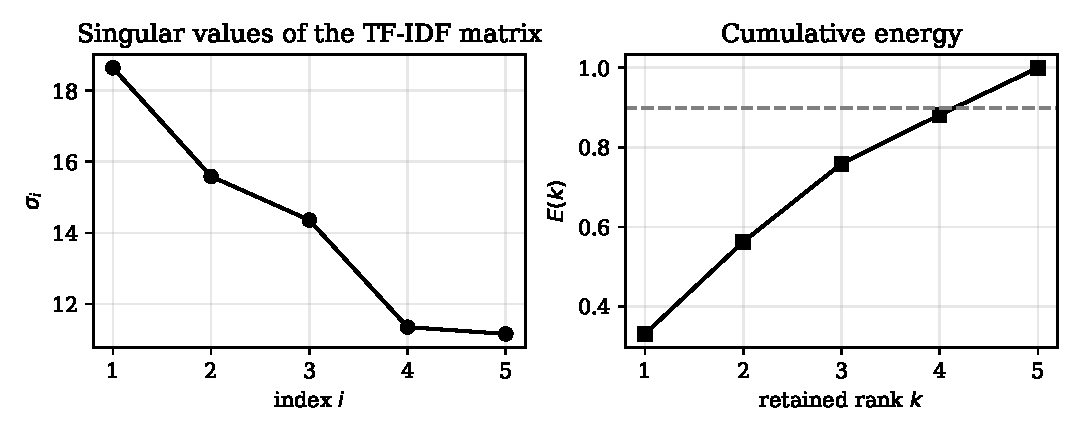
\includegraphics[width=0.95\textwidth]{figures/experiment1/spectrum.pdf}
\caption{Left: the singular values of the TF-IDF matrix. Right: cumulative energy $E(k)$; the dashed line marks the default target $0.90$.}\label{fig:spectrum}
\end{figure}

\subsection{Document similarity}

Table~\ref{tab:pairs} lists the cosine similarity of every pair of documents under the baseline and under LSA with $k=2,3,4$. The column for $k=5$ is left out because it coincides with the baseline: the largest difference over the ten pairs is $9.4\times10^{-16}$, which is the exact-arithmetic identity of Proposition~\ref{prop:cos}(a) showing up in floating point. Table~\ref{tab:groups} summarises the same data by topic, and Figure~\ref{fig:heat} shows the full matrices.

\begin{table}[H]
\centering
\caption{Cosine similarity of all document pairs: TF-IDF baseline and LSA at ranks $k=2,3,4$. The first two rows are same-topic pairs.}\label{tab:pairs}
\begin{tabular}{@{}lcccc@{}}
\toprule
Document pair & TF-IDF cosine & LSA, $k=2$ & LSA, $k=3$ & LSA, $k=4$\\
\midrule
coffee--cafe & 0.3760 & 0.9947 & 0.9823 & 0.5319\\
hike--camping & 0.3635 & 0.9988 & 0.9941 & 0.7109\\
\midrule
coffee--hike & 0.1046 & 0.0974 & 0.1501 & 0.2891\\
coffee--camping & 0.0849 & 0.0481 & 0.1169 & -0.0378\\
coffee--music & 0.0843 & 0.2771 & 0.0550 & 0.0656\\
cafe--hike & 0.1006 & 0.1994 & 0.1783 & -0.0881\\
cafe--camping & 0.0978 & 0.1507 & 0.1264 & 0.2887\\
cafe--music & 0.1410 & 0.3745 & 0.2408 & 0.1802\\
hike--music & 0.1658 & 0.9833 & 0.2378 & 0.2325\\
camping--music & 0.1345 & 0.9731 & 0.1351 & 0.1135\\
\bottomrule
\end{tabular}
\end{table}

\textbf{Baseline.} The TF-IDF cosines are small throughout, between 0.084 and 0.166 for different-topic pairs, and only 0.376 and 0.363 for the two same-topic pairs. Related passages share only a handful of content words, and what they share is partly function words, so even clearly related documents look only mildly similar.

\textbf{Rank two.} At $k=2$ the same-topic pairs are almost parallel (0.995 and 0.999), but the music document is also pulled onto the outdoor documents: its cosine is 0.983 with the hike passage and 0.973 with the camping passage, while it stays at 0.277 and 0.375 with the coffee passages (Figure~\ref{fig:plane}). For this collection, projection onto the first two singular directions makes the music and outdoor document vectors nearly parallel. Including the third component improves their separation.

\textbf{Rank three.} At $k=3$ the same-topic pairs remain close to parallel (0.982 and 0.994), and every different-topic pair stays below 0.241. The three topics now each have their own direction, and the contrast between same-topic and different-topic pairs is much sharper than in the baseline (Table~\ref{tab:groups}).

\textbf{Rank four.} At $k=4$ the similarities move back towards the baseline: the same-topic pairs fall to 0.532 and 0.711, and two different-topic pairs (coffee--camping at -0.038, cafe--hike at -0.088) become slightly negative. Negative values here are angles larger than a right angle in the reduced space; they do not mean that the documents contradict each other.

\begin{table}[H]
\centering
\caption{Mean cosine similarity for the two same-topic pairs and for the eight different-topic pairs.}\label{tab:groups}
\begin{tabular}{@{}lcc@{}}
\toprule
Representation & Same-topic pairs (mean) & Different-topic pairs (mean)\\
\midrule
TF-IDF baseline & 0.3697 & 0.1142\\
LSA, $k=2$ & 0.9967 & 0.3879\\
LSA, $k=3$ & 0.9882 & 0.1550\\
LSA, $k=4$ & 0.6214 & 0.1305\\
LSA, $k=5$ & 0.3697 & 0.1142\\
\bottomrule
\end{tabular}
\end{table}

\begin{figure}[H]
\centering
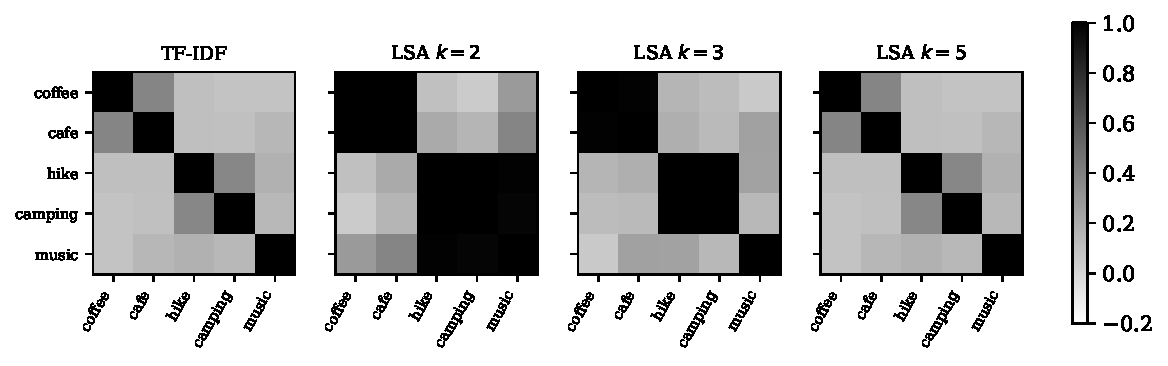
\includegraphics[width=\textwidth]{figures/experiment1/heatmaps.pdf}
\caption{Pairwise cosine similarities for the five documents: TF-IDF baseline and LSA with $k=2,3,5$. Darker cells mean higher cosine.}\label{fig:heat}
\end{figure}

\begin{figure}[H]
\centering
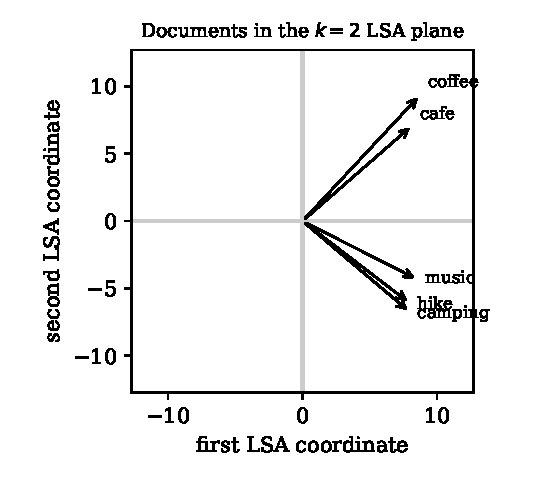
\includegraphics[width=0.55\textwidth]{figures/experiment1/plane2d.pdf}
\caption{The five documents as vectors in the $k=2$ LSA plane. Cosine similarity compares the angles between these arrows.}\label{fig:plane}
\end{figure}

\textbf{What the leading directions capture.} Table~\ref{tab:dirs} lists the terms that carry the largest entries of the first three left singular vectors. The first direction is dominated by very frequent function words (\emph{the}, \emph{and}, \emph{a}, \emph{with}); this is the expected consequence of not removing stop-words, because their large counts give them large entries in $A$ even though idf is at least one. The second direction contrasts the vocabulary of the coffee passages (\emph{with}, \emph{beans}, \emph{brewing}, \emph{cake}) with the word \emph{we}, which occurs in the camping passage. The third direction is carried by words specific to the music passage (\emph{audience}, \emph{beat}, \emph{applauded}, \emph{concert}), again opposed to \emph{we}. This is consistent with the rank experiment: in the third LSA coordinate the music document has by far the largest magnitude (-11.97 against at most 6.15 for the other four), so including a third dimension is what gives the music document its own direction.

\begin{table}[H]
\centering
\caption{Terms with the largest loadings (entries of $u_i$) on the first three left singular vectors. The sign of a singular vector is arbitrary; only relative signs matter.}\label{tab:dirs}
\small
\begin{tabular}{@{}cp{0.82\textwidth}@{}}
\toprule
$i$ & Leading terms (loading)\\
\midrule
1 & \emph{the} (+0.43), \emph{and} (+0.24), \emph{a} (+0.24), \emph{with} (+0.19), \emph{water} (+0.15), \emph{before} (+0.14)\\
2 & \emph{with} (+0.28), \emph{beans} (+0.20), \emph{brewing} (+0.20), \emph{we} (-0.15), \emph{cake} (+0.13), \emph{coffee} (+0.13)\\
3 & \emph{we} (+0.16), \emph{audience} (-0.15), \emph{beat} (-0.15), \emph{applauded} (-0.15), \emph{during} (-0.15), \emph{evening} (-0.15)\\
\bottomrule
\end{tabular}
\end{table}

\subsection{Second case study: a longer administrative document collection}

To examine the same implementation on a collection with longer passages and a larger vocabulary, I ran it on five additional documents in \texttt{Data/LongSamples}. The files concern the evening campus shuttle, library archive digitisation, and a student society treasury handover. The shuttle pair (06, 07) and archive pair (08, 09) are treated as same-topic pairs for descriptive comparison; the treasury document (10) is a singleton. These groupings are reference labels for this small experiment, not independent relevance judgements.

\begin{table}[H]
\centering
\caption{Description of the second document collection.}\label{tab:dataset2}
\begin{tabular}{@{}p{0.25\textwidth}p{0.68\textwidth}@{}}
\toprule
Field & Details\\
\midrule
Documents & 06 shuttle proposal.txt, 07 shuttle feedback.txt, 08 archive proposal.txt, 09 archive workflow.txt, and 10 club treasury.txt.\\
Document lengths & 456, 443, 446, 446 and 441 tokens respectively, after the cleaning and tokenisation in Section~2.3.1.\\
Topical grouping & Shuttle: 06 and 07; archive: 08 and 09; treasury: 10 (singleton). Used only to summarise pairwise similarities.\\
Vocabulary and matrix size & 813 distinct terms; the TF-IDF matrix is $813\times5$ with 1,281 nonzero entries.\\
Provenance and limitations & The five text files were generated by ChatGPT (OpenAI) for this project. They are synthetic, not collected from an institution, and do not provide independent relevance labels.\\
Preprocessing & Identical to the first experiment: \texttt{[a-z]+} tokenisation, raw term counts, $\mathrm{idf}_i=1+\ln(N/\mathrm{df}_i)$, and no stop-word removal or stemming.\\
\bottomrule
\end{tabular}
\end{table}

The custom Gram-matrix implementation returns numerical rank $r=5$. Its singular values are
\[
\sigma_1,\ldots,\sigma_5=115.6399,\ 58.8705,\ 52.0761,\ 41.5334,\ 36.8844.
\]
The relative reconstruction error is $4.90\times10^{-16}$, while the orthogonality errors are $e_U=3.71\times10^{-15}$ and $e_V=1.07\times10^{-15}$. The relative error in the identity $\sum_i\sigma_i^2=\norm{A}_F^2$ is $8.04\times10^{-16}$. Thus the custom implementation again reconstructs this TF-IDF matrix to double-precision accuracy.

\begin{table}[H]
\centering
\caption{Retained energy, relative Frobenius error and retained condition number for the second collection.}\label{tab:energy2}
\begin{tabular}{@{}ccccc@{}}
\toprule
$k$ & $E(k)$ & $\norm{A-A_k}_F/\norm{A}_F$ & $\sqrt{1-E(k)}$ & $\sigma_1/\sigma_k$\\
\midrule
1 & 0.5908 & 0.6397 & 0.6397 & 1.000\\
2 & 0.7439 & 0.5061 & 0.5061 & 1.964\\
3 & 0.8637 & 0.3692 & 0.3692 & 2.221\\
4 & 0.9399 & 0.2452 & 0.2452 & 2.784\\
5 & 1.0000 & 0.0000 & 0.0000 & 3.135\\
\bottomrule
\end{tabular}
\end{table}

The default 90\% energy rule therefore selects $k=4$; an 80\% target selects $k=3$. Figure~\ref{fig:spectrum2} shows the more pronounced decay in this collection than in the first experiment. Four components retain 93.99\% of the energy, while three retain 86.37\%.

\begin{figure}[H]
\centering
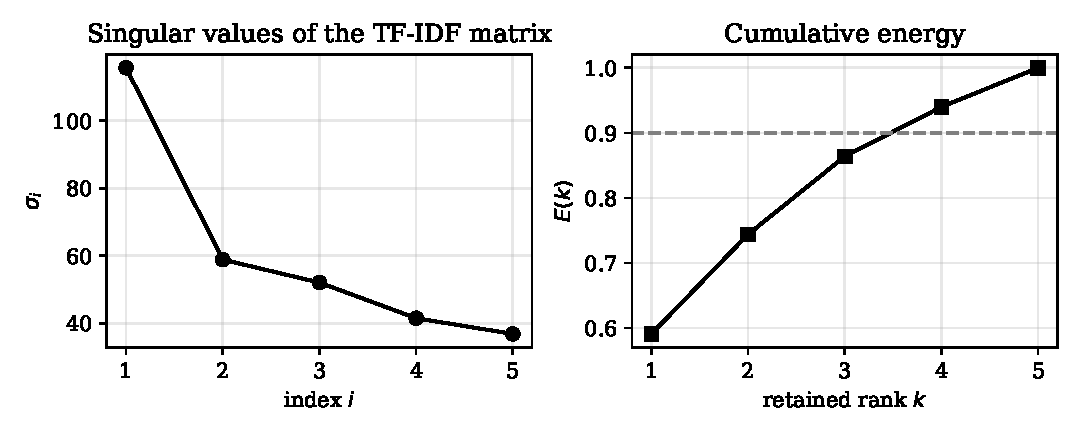
\includegraphics[width=0.95\textwidth]{figures/experiment2/spectrum.pdf}
\caption{Singular values and cumulative spectral energy for the second TF-IDF matrix. The dashed line marks the 90\% target.}\label{fig:spectrum2}
\end{figure}

Table~\ref{tab:pairs2} compares all ten document pairs. The $k=5$ column is omitted because retaining all five components reproduces the TF-IDF cosine similarities, as Proposition~\ref{prop:cos}(a) predicts.

\begin{table}[H]
\centering
\caption{Pairwise cosine similarities for the second collection.}\label{tab:pairs2}
\small
\begin{tabular}{@{}p{0.39\textwidth}cccc@{}}
\toprule
Document pair & TF-IDF & LSA $k=2$ & LSA $k=3$ & LSA $k=4$\\
\midrule
Shuttle proposal--feedback & 0.6762 & 0.9990 & 0.9989 & 0.7677\\
Shuttle proposal--archive proposal & 0.4172 & 0.4995 & 0.4840 & 0.5415\\
Shuttle proposal--archive workflow & 0.4359 & 0.6031 & 0.5879 & 0.3903\\
Shuttle proposal--treasury & 0.4645 & 0.7093 & 0.5250 & 0.4822\\
Shuttle feedback--archive proposal & 0.3753 & 0.4599 & 0.4526 & 0.3284\\
Shuttle feedback--archive workflow & 0.4778 & 0.5665 & 0.5578 & 0.5976\\
Shuttle feedback--treasury & 0.4622 & 0.6768 & 0.4900 & 0.4699\\
Archive proposal--workflow & 0.6059 & 0.9923 & 0.9918 & 0.8054\\
Archive proposal--treasury & 0.4310 & 0.9650 & 0.4732 & 0.4512\\
Archive workflow--treasury & 0.4761 & 0.9901 & 0.5372 & 0.5106\\
\bottomrule
\end{tabular}
\end{table}

\begin{table}[H]
\centering
\caption{Mean cosine similarities for designated same-topic pairs and different-topic pairs in the second collection.}\label{tab:groups2}
\begin{tabular}{@{}lcc@{}}
\toprule
Representation & Same-topic mean & Different-topic mean\\
\midrule
TF-IDF baseline & 0.6411 & 0.4425\\
LSA, $k=2$ & 0.9956 & 0.6838\\
LSA, $k=3$ & 0.9954 & 0.5135\\
LSA, $k=4$ & 0.7865 & 0.4715\\
LSA, $k=5$ & 0.6411 & 0.4425\\
\bottomrule
\end{tabular}
\end{table}

Figure~\ref{fig:heat2} displays the similarity matrices. At $k=2$, the treasury document has cosine similarities 0.9650 and 0.9901 with the two archive documents, even though it is assigned to a different topic. This is a concrete example of a low-rank representation making unrelated documents appear close. At $k=3$, these two scores fall to 0.4732 and 0.5372, while the shuttle and archive pairs remain at 0.9989 and 0.9918. The mean gap between designated same-topic and different-topic pairs is therefore larger at $k=3$ than in the TF-IDF baseline. However, this rank was inspected against the known grouping and should not be interpreted as a validated model-selection result.

\begin{figure}[H]
\centering
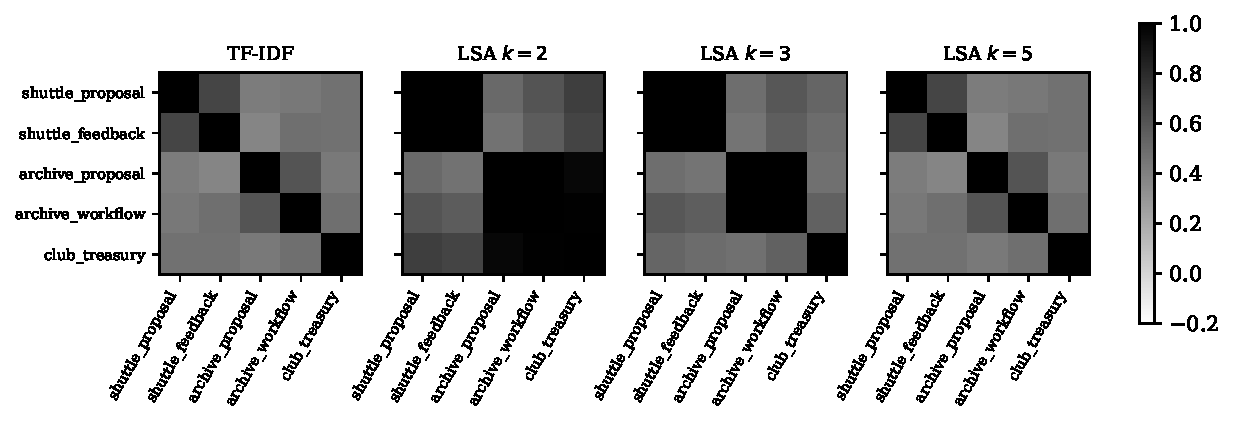
\includegraphics[width=\textwidth]{figures/experiment2/heatmaps.pdf}
\caption{TF-IDF and LSA cosine-similarity matrices for the second collection at $k=2$, $k=3$ and full rank.}\label{fig:heat2}
\end{figure}

The two-dimensional projection in Figure~\ref{fig:plane2} is included as a geometric view of the $k=2$ coordinates. It must be read alongside the heatmap: a two-dimensional projection can make the treasury and archive documents appear close, which is consistent with the false similarities just discussed.

\begin{figure}[H]
\centering
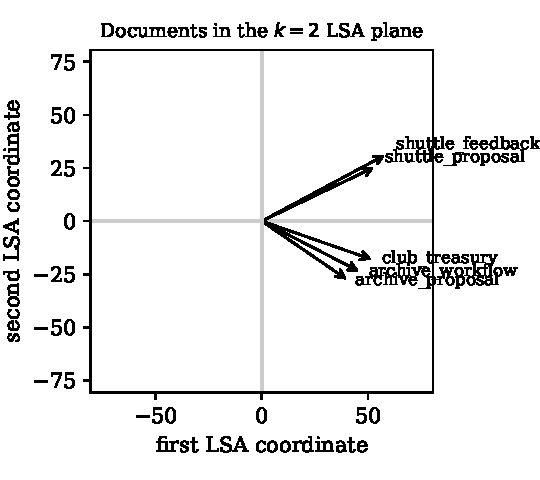
\includegraphics[width=0.55\textwidth]{figures/experiment2/plane2d.pdf}
\caption{The five documents represented in the first two LSA coordinates of the second collection.}\label{fig:plane2}
\end{figure}

The first left singular vector is dominated by common function words such as \emph{the}, \emph{a}, and \emph{and}, reflecting the decision not to remove stop-words. The second direction has prominent shuttle-related terms such as \emph{route}, \emph{gate}, \emph{timetable} and \emph{shuttle}, contrasted with \emph{catalogue}. The third direction includes \emph{handover}, \emph{expense} and \emph{authorised}, which are associated with the treasury document. These loadings offer one interpretation of why the third component helps separate the treasury document from the archive pair.

\subsection{Observations and limits of the experiment}

These two case studies illustrate the method; they do not validate it. Each collection contains only five documents. All ten text files across the two collections were generated by ChatGPT (OpenAI); they are synthetic, not records collected from an institution, and do not constitute an independent benchmark. The topic groupings are reference groupings used to interpret the cosine scores, not independent relevance labels.

The two collections also show that the effect of truncation depends on the data. In the first collection, the 90\% energy rule selects full rank and does not reduce dimension. In the second, it selects $k=4$, while $k=3$ gives a larger separation between the designated same-topic and different-topic means in this particular collection. At $k=2$, the second collection also exhibits false similarities between the treasury document and the archive documents. These observations do not establish that either rank is generally preferable; the ranks were inspected against the known groupings. With real retrieval data, $k$ should be selected using labelled validation queries and compared using retrieval metrics.

Both experiments use the same preprocessing, including no stop-word removal, stemming or minimum document-frequency filter. The leading singular directions therefore reflect common function words as well as topic-related vocabulary. Changing preprocessing would change the matrix and its spectrum, but those alternatives have not been tested here. Singular vectors are defined only up to sign (and rotations within repeated singular-value subspaces), so the interpretation of individual loading signs is not unique. The numerical values were produced with the implementation and environment described in the report; another platform or library version may change the final digits of rounding-level errors.

\subsection{Third experiment: labelled 20 Newsgroups sample}
\label{sec:precision}

\subsubsection{Data and reproducible sampling}
The real-text experiment uses \texttt{fetch\_20newsgroups} from scikit-learn \cite{newsgroups}. It selects the by-date training subset with \texttt{shuffle=False} and requests removal of headers, footers and quotes. These loader filters reduce obvious metadata cues; they should not be interpreted as a guarantee that every such cue is removed. Five categories are used: \texttt{comp.graphics}, \texttt{rec.autos}, \texttt{rec.sport.baseball}, \texttt{sci.med} and \texttt{sci.space}. After the project's cleaning and tokenisation, documents with fewer than 30 tokens are excluded. A NumPy random generator with seed 42 samples 50 eligible documents per category without replacement, giving 250 documents.

The selected documents are written to \texttt{Data/20newsgroups/documents/}; \texttt{labels.csv} records filenames, categories and source identifiers. The loader then sorts filenames and the category labels are aligned to that order. The same custom preprocessing and raw-count TF-IDF formula as in the two earlier experiments are used, with no stop-word removal or column normalisation before SVD. The resulting matrix is $A\in\R^{6479\times250}$, so the engine solves a $250\times250$ Gram eigenproblem. Its numerical rank is 250.

\subsubsection{Evaluation protocol}
Let $q$ denote the number of retrieved neighbours and $k$ the retained SVD rank; these are different parameters. For document $i$, let $R_q(i)$ contain the indices of the $q$ highest-cosine other documents. With category label $y_i$,
\[
 P_i@q=\frac{1}{q}\sum_{j\in R_q(i)}\mathbf{1}[y_j=y_i],
 \qquad \overline{P@q}=\frac{1}{N}\sum_{i=1}^{N}P_i@q.
\]
The experiment uses $q=5$. Self-matches are removed before ranking, and exact ties follow filename order through a stable sort. Negative similarities are ranked by their numerical value, not their absolute magnitude. A category match is a proxy for relevance. With 50 documents per category, each query has 49 relevant candidates, and precision at five can attain one.

TF-IDF is compared against LSA at fixed ranks 5, 10, 20 and 50, with rank 250 included as a cosine-preservation check. The 90\% energy rule used by the CLI does not select these ranks. Every document serves as a query against the other 249 documents in the same fitted collection. No held-out queries or separate rank-selection split are used. This is an exploratory within-collection neighbour evaluation, not classification accuracy or evidence of generalisation to unseen queries.

\subsubsection{Results and interpretation}
\begin{table}[H]
\centering
\caption{Recorded results on the balanced 250-document sample. Energy is relative to the full retained numerical spectrum.}
\label{tab:bigresults}
\begin{tabular}{@{}lrr@{}}
\toprule
Representation & Mean precision@5 & Retained energy\\
\midrule
TF-IDF & 0.4976 & ---\\
LSA k=5 & 0.2848 & 38.80\%\\
LSA k=10 & 0.4296 & 49.16\%\\
LSA k=20 & 0.4864 & 61.14\%\\
LSA k=50 & 0.4928 & 76.89\%\\
LSA k=250 & 0.4976 & 100.00\%\\
\bottomrule
\end{tabular}
\end{table}

No tested reduced rank exceeds the TF-IDF baseline. At rank 50, the score is 0.0048 below the baseline (0.48 percentage points), while each document uses 50 LSA coordinates instead of 6,479 term coordinates. This comparison concerns representation dimension only: no end-to-end runtime or peak-memory improvement was measured, and the implementation still forms dense matrices and computes the compact SVD before truncating. Full-rank LSA matches the TF-IDF precision, as predicted by the cosine-preservation identity.

The committed run reports a relative reconstruction error of $1.8831\times10^{-15}$ and a maximum absolute difference between full-rank LSA and TF-IDF cosines of $2.2260\times10^{-14}$. The retained condition number at full rank is approximately 30.38. An independent rerun reproduced all six mean precision scores to four decimal places; small changes in floating-point residuals are expected across environments.

\begin{figure}[H]
\centering
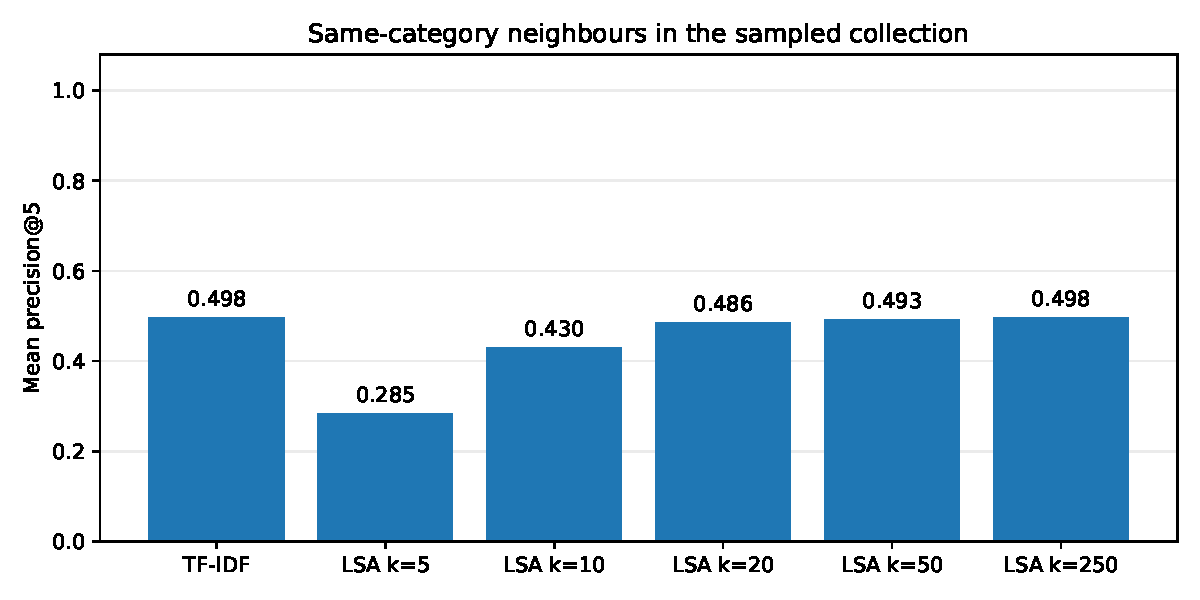
\includegraphics[width=0.95\textwidth]{figures/experiment_big/precision_at_5.pdf}
\caption{Mean precision at five neighbours for TF-IDF and the tested LSA ranks.}
\label{fig:bigprecision}
\end{figure}

\begin{figure}[H]
\centering
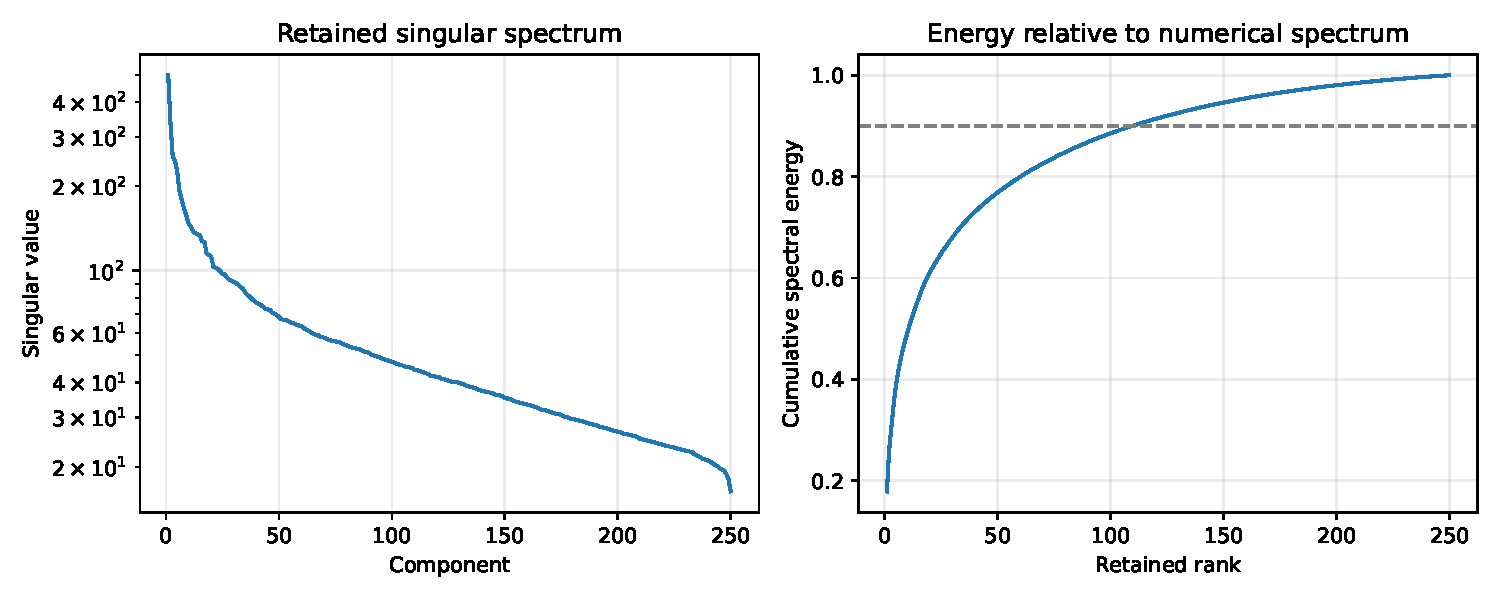
\includegraphics[width=0.95\textwidth]{figures/experiment_big/spectrum.pdf}
\caption{Singular spectrum and cumulative energy for the 250-document collection. Retained energy and neighbour precision measure different properties.}
\label{fig:bigspectrum}
\end{figure}

\subsubsection{Reproduction and scope}
Run \texttt{python -m experiments.experiment\_big} from the repository root after installing the dependencies. The first run downloads the dataset; subsequent runs can use the local cache. The generated text collection is excluded from version control. Changing the sampling configuration requires moving any previous document folder aside because unexpected files are rejected rather than silently mixed into the new sample.

The driver writes \texttt{figures/experiment\_big/results.json} and PDF/PNG figures. Its JSON contains sampling settings, category labels, document names, SHA-256 hashes of the input files, the numerical spectrum, precision for individual documents and categories, reconstruction diagnostics and package versions. The committed run records Python 3.13.16, NumPy 2.5.3, Matplotlib 3.11.2 and scikit-learn 1.9.1. These are recorded run versions, not exact installation requirements. The repository's environment files define its dependency requirements.

Only one balanced sample and four reduced ranks were evaluated. There are no confidence intervals or repeated sampling trials, and the small rank-50 difference should not be interpreted as statistically established superiority or inferiority. The category labels are not query-specific relevance judgements. A stronger evaluation would use separate validation and query sets, multiple seeds, and additional retrieval measures.

\chapter{Conclusions and Future Work}

The project constructs a compact SVD using the eigendecomposition of the smaller Gram matrix and applies it to document similarity. The Eckart--Young theorem explains the optimality of truncation for matrix reconstruction, while the experiments show why this does not imply optimal retrieval. In the two synthetic collections, truncation can increase same-topic cosines but can also merge unrelated documents. These examples illustrate the geometry rather than establish retrieval quality.

The completed 20 Newsgroups experiment adds a labelled evaluation on 250 real documents. TF-IDF obtains mean precision@5 of 0.4976; the tested reduced LSA ranks give 0.2848, 0.4296, 0.4864 and 0.4928. Full-rank LSA reproduces the baseline. The principal empirical finding is therefore that reduced rank did not improve mean neighbour precision on this sample, although rank 50 preserved much of the baseline score in fewer coordinates. Reconstruction and full-rank cosine checks agree with the theoretical identities to near floating-point precision.

The main limitations are the accuracy loss from forming Gram matrices, dense storage, the loss of word order, and sensitivity to preprocessing and retained rank. The labelled evaluation is within one fitted collection and uses one seed, so it does not establish performance on unseen queries. Future work should separate validation from evaluation, repeat sampling, examine stop-word removal and alternative weighting, and measure runtime and memory as well as retrieval quality. A direct SVD method such as bidiagonalisation or one-sided Jacobi rotations would provide a useful numerical comparison. New query vectors could be projected as $U_k\T q$ after using the fitted vocabulary and IDF weights.

\section*{Code availability}
The source repository is listed in \cite{repo}. Its code is distributed under the MIT License; the root \texttt{LICENSE} file contains the applicable terms and copyright notice. Third-party dependencies and the downloaded dataset retain their own applicable terms. The report's appendix reproduces the current implementation of the five core modules and all three experiment drivers. Unit-test source is omitted.

\chapter*{Generative AI Usage Declaration}
\addcontentsline{toc}{chapter}{Generative AI Usage Declaration}

I declare the following use of Generative AI tools in the preparation of this project.

\textbf{ChatGPT (OpenAI).} Used for conceptual clarification, test assistance, debugging, mathematical exposition, and report editing and formatting. ChatGPT also generated the ten synthetic text documents used in the first two experiments: the five documents in the first collection and the five documents in the second collection. These documents are synthetic examples; they are not records collected from an institution and do not form an independent benchmark. The third experiment uses existing 20 Newsgroups posts retrieved through scikit-learn, not AI-generated documents.

\textbf{Claude (Anthropic).} Used to rewrite and restructure the earlier draft prepared on Google Docs into the present LaTeX report. The extent of this use is substantial drafting and editing assistance.

All figures, plots and diagrams in this report were generated using Matplotlib from the numerical output of the project code. No externally sourced or AI-generated image assets are included.

\textbf{Statement.} During the preparation of this report, I used ChatGPT and Claude to clarify concepts, assist with code, and draft and format the report as described above. I reviewed and edited the content as needed and take responsibility for the submitted report.

\begin{thebibliography}{99}
\addcontentsline{toc}{chapter}{Bibliography}

\bibitem{lectures} MAC F211 course lecture material, \emph{Lec\_26-27} and \emph{Lec\_28-29} (Singular Value Decomposition), Department of Mathematics, BITS Pilani, K K Birla Goa Campus, 2026.

\bibitem{lay} D. C. Lay, S. R. Lay and J. J. McDonald, \emph{Linear Algebra and Its Applications}, 5th ed., Pearson Education, 2023.

\bibitem{strang} G. Strang, \emph{Linear Algebra and Its Applications}, 4th ed., Cengage India Private Limited, 2005.

\bibitem{deerwester} S. Deerwester, S. T. Dumais, G. W. Furnas, T. K. Landauer and R. Harshman, ``Indexing by latent semantic analysis,'' \emph{Journal of the American Society for Information Science}, 41(6), 391--407, 1990.

\bibitem{eckartyoung} C. Eckart and G. Young, ``The approximation of one matrix by another of lower rank,'' \emph{Psychometrika}, 1(3), 211--218, 1936.

\bibitem{golubvanloan} G. H. Golub and C. F. Van Loan, \emph{Matrix Computations}, 4th ed., Johns Hopkins University Press, 2013.

\bibitem{Manning}
C. D. Manning, P. Raghavan and H. Sch\"utze,
\emph{Introduction to Information Retrieval},
Cambridge University Press, 2008, Chapters 6 and 18.

\bibitem{numpyeigh} NumPy Developers, \texttt{numpy.linalg.eigh}, NumPy documentation. \url{https://numpy.org/doc/stable/reference/generated/numpy.linalg.eigh.html}. Accessed 1 November 2026.

\bibitem{numpysvd} NumPy Developers, \texttt{numpy.linalg.svd}, NumPy documentation. \url{https://numpy.org/doc/stable/reference/generated/numpy.linalg.svd.html}. Accessed 1 November 2026.

\bibitem{girdher} H. Girdher, ``TDM (Term Document Matrix) and DTM (Document Term Matrix),'' Analytics Vidhya, Medium, 30 July 2021. \url{https://medium.com/analytics-vidhya/tdm-term-document-matrix-and-dtm-document-term-matrix-8b07c58957e2}. Accessed 23 October 2026.

\bibitem{repo} Pranjal Kumar, \emph{SVD Subtext}, GitHub repository, 2026. \url{https://github.com/pranjalkumar0001/SVD_subtext}.

\bibitem{newsgroups} Scikit-learn Developers, \texttt{fetch\_20newsgroups}, scikit-learn documentation. \url{https://scikit-learn.org/stable/modules/generated/sklearn.datasets.fetch_20newsgroups.html}. Accessed 19 November 2026.

\end{thebibliography}

\appendix
\chapter{Programming Code}
This appendix contains the five core modules and all three experiment drivers from the project repository. Unit-test source is omitted. The Conda environment specifies Python 3.13; the dependencies include NumPy, Matplotlib, pytest and scikit-learn. The core application uses NumPy; Matplotlib supplies figures and scikit-learn supplies the real-text dataset. Run commands from the repository root:
\begin{verbatim}
python -m src.main Data/Samples --k 3
python -m experiments.experiment1
python -m experiments.experiment2
python -m experiments.experiment_big
\end{verbatim}
Each experiment writes results to its own subdirectory of \texttt{figures/}, so running one does not overwrite another experiment's JSON output.

\section{Document loading}
\noindent File: \texttt{src/data\_loader.py}
\begin{lstlisting}
from pathlib import Path

def load_txt_documents(folder_path: str | Path) -> dict[str, str]:
    """
    Loads all .txt documents from the specified folder and returns a dictionary
    where keys are filenames (with extension) and values are the corresponding
    document contents.

    Args:
        folder_path (str | Path): The path to the folder containing .txt files."""

    folder =  Path(folder_path)
    if not folder.exists():
        raise FileNotFoundError(f"The provided path '{folder_path}' is not a valid directory.")
    if not folder.is_dir():
        raise NotADirectoryError(f"The provided path '{folder_path}' is not a valid directory.")

    files = sorted(
        (
            path
            for path in folder.iterdir()
            if path.is_file() and path.suffix.lower() == ".txt"
        ),
        key=lambda path: path.name)
    if not files:
        raise ValueError(f"No .txt files found in the directory '{folder_path}'.")

    doc_names = [file.name for file in files]
    doc_contents = [file.read_text(encoding="utf-8-sig") for file in files]
    return dict(zip(doc_names, doc_contents))
\end{lstlisting}

\section{Text preprocessing and TF-IDF}
\noindent File: \texttt{src/preprocessing.py}
\begin{lstlisting}
import re
import numpy as np

def clean_text(text: str) -> str:
    """
    Cleans the input text by removing unwanted characters, urls, email addresses and formatting.

    Args:
        text (str): The input text to be cleaned.

    Returns:
        str: The cleaned text.
    """
    if not isinstance(text, str):
        raise TypeError("Input must be a string.")

    # Remove URLs
    text = re.sub(r"\b(?:https?://|www\.)\S+", " ", text, flags=re.IGNORECASE)

    # Remove email addresses
    text = re.sub(r"\b[A-Z0-9._%+-]+@[A-Z0-9.-]+\.[A-Z]{2,}\b"," ",text,flags=re.IGNORECASE)

    # Remove unwanted characters (keeping only alphanumeric and spaces)
    text = re.sub(r"[^a-zA-Z0-9\s]", " ", text)

    # Normalize whitespace
    text = re.sub(r"\s+", " ", text).strip()

    return text.lower()


def tokenize(text: str) -> list[str]:
    """Return lowercase English word tokens, preserving repetitions."""
    if not isinstance(text, str):
        raise TypeError("text must be a string")

    return re.findall(r"[a-z]+", text.lower())


def build_count_matrix(documents: dict[str, str]) -> tuple[np.ndarray, list[str], list[str]]:
    """Return counts, row vocabulary, and column document names.

    Columns preserve the input dictionary's insertion order.
    """
    if not documents:
        raise ValueError("No documents provided.")

    doc_names = list(documents)
    tokenized_documents = [tokenize(clean_text(documents[name])) for name in doc_names]

    unique_words = set()
    for tokens in tokenized_documents:
        unique_words.update(tokens)

    vocabulary = sorted(unique_words)

    if not vocabulary:
        raise ValueError("No tokens found in the documents.")

    word_to_index = {word: index for index, word in enumerate(vocabulary)}

    matrix = np.zeros((len(vocabulary), len(doc_names)), dtype=np.float64)

    for doc_index, tokens in enumerate(tokenized_documents):
        for word in tokens:
            word_index = word_to_index[word]
            matrix[word_index, doc_index] += 1

    return matrix, vocabulary, doc_names


def compute_tfidf(counts: np.ndarray) -> tuple[np.ndarray, np.ndarray]:
    """Return the TF-IDF matrix and IDF vector.

    Rows represent terms; columns represent documents.

    TF = raw count
    IDF = 1 + ln(number_of_documents / document_frequency)

    The input matrix is not modified.
    """
    counts = np.asarray(counts, dtype=np.float64)

    if counts.ndim != 2:
        raise ValueError("Counts must be a two-dimensional matrix.")

    if 0 in counts.shape:
        raise ValueError("Counts must contain at least one term and one document.")

    if not np.all(np.isfinite(counts)):
        raise ValueError("Counts must contain only finite values.")

    if np.any(counts < 0):
        raise ValueError("Counts cannot be negative.")

    number_of_documents = counts.shape[1]

    # Number of documents containing each term.
    document_frequency = np.count_nonzero(counts > 0, axis=1)

    if np.any(document_frequency == 0):
        raise ValueError("Each vocabulary term must occur in at least one document.")

    idf = 1 + np.log(number_of_documents / document_frequency)

    # Broadcast one IDF weight per row across all document columns.
    tfidf = counts * idf[:, None]

    return tfidf, idf
\end{lstlisting}

\section{Gram-matrix SVD}
\noindent File: \texttt{src/SVD.py}
\begin{lstlisting}
import numpy as np


def svd_from_gram(matrix: np.ndarray) -> tuple[np.ndarray, np.ndarray, np.ndarray]:
    """Compute a compact SVD using the smaller Gram matrix.

    Parameters
    ----------
    matrix : np.ndarray Nonempty, finite, real matrix with shape (m, n).

    Returns
    -------
    U : np.ndarray, Left singular vectors, shape (m, r), orthonormal.
    Sigma : np.ndarray, Positive singular values in descending order, shape (r, r), diagonal matrix.
    Vt : np.ndarray, Transposed right singular vectors, shape (r, n), orthonormal.

    Here r is the estimated numerical rank. Reconstruction:
        matrix ≈ U @ Sigma @ Vt

    Notes
    -----
    Gram-matrix formation reduces accuracy for small singular values.
    Eigenvalues below a numerical tolerance are discarded.
    The input is not modified.
    """
    raw = np.asarray(matrix)

    if np.iscomplexobj(raw):
        raise ValueError("Only real-valued matrices are supported.")

    A = np.asarray(raw, dtype=np.float64)

    if A.ndim != 2:
        raise ValueError("Input must be a two-dimensional matrix.")

    if 0 in A.shape:
        raise ValueError("Input must have at least one row and column.")

    if not np.all(np.isfinite(A)):
        raise ValueError("Input must contain only finite values.")

    m, n = A.shape
    # Scale to reduce overflow risk when forming the Gram matrix.
    scale = np.max(np.abs(A))
    
    # Compact SVD of a zero matrix has rank zero.
    if scale == 0:
        return (
            np.empty((m, 0), dtype=np.float64),
            np.empty((0, 0), dtype=np.float64),
            np.empty((0, n), dtype=np.float64),
        )

    B = A / scale

    # Choose the smaller symmetric eigenvalue problem.
    if m >= n:
        gram = B.T @ B
    else:
        gram = B @ B.T

    eigenvalues, eigenvectors = np.linalg.eigh(gram)

    # Sort eigenvalues and their corresponding eigenvector columns.
    order = np.argsort(eigenvalues)[::-1]
    eigenvalues = eigenvalues[order]
    eigenvectors = eigenvectors[:, order]

    # Numerical rank threshold at the Gram-matrix scale.
    # The factor 10 is a conservative heuristic, not an exact bound.
    eps = np.finfo(np.float64).eps
    tolerance = 10.0 * eps * max(m, n) * eigenvalues[0]

    if np.any(eigenvalues < -tolerance):
        raise np.linalg.LinAlgError(
            "Gram matrix has a significantly negative eigenvalue."
        )

    # Exclude numerical zeros and tiny negative round-off errors.
    keep = eigenvalues > tolerance
    s_scaled = np.sqrt(eigenvalues[keep])
    vectors = eigenvectors[:, keep]

    # Recover the other singular-vector factor.
    if m >= n:
        V = vectors
        U = (B @ V) / s_scaled
    else:
        U = vectors
        V = (B.T @ U) / s_scaled

    # Choose paired signs so each U column's largest entry
    # in absolute value is positive.
    columns = np.arange(U.shape[1])
    largest_rows = np.argmax(np.abs(U), axis=0)
    signs = np.where(
        U[largest_rows, columns] < 0.0,
        -1.0,
        1.0,
    )

    U = U * signs
    V = V * signs

    # Restore singular values to the original scale.
    with np.errstate(over="ignore"):
        s = s_scaled * scale
        Sigma = np.diag(s)

    if not np.all(np.isfinite(s)):
        raise FloatingPointError(
            "Singular values exceed the float64 numerical range."
        )

    return U, Sigma, V.T
\end{lstlisting}

\section{Rank selection and similarity}
\noindent File: \texttt{src/similarity.py}
\begin{lstlisting}
import numpy as np


def suggest_k(Sigma: np.ndarray,energy_target: float = 0.90) -> int:
    """
    Return the smallest k that retains the requested spectral energy.

    Sigma must be a diagonal matrix of positive singular values,
    sorted in descending order, as returned by the SVD engine.

    Energy is measured relative to the singular values retained by
    the engine. This is a reconstruction heuristic, not a guarantee
    of better document similarity.
    """
    if not 0 < energy_target <= 1:
        raise ValueError("energy_target must be in (0, 1].")

    singular_values = np.diag(Sigma) # get singular values from diagonal matrix

    if singular_values.size == 0:
        raise ValueError("Cannot suggest k for a rank-zero matrix.")

    # Scaling prevents overflow when squaring large singular values.
    relative_energy = (singular_values / singular_values[0]) ** 2

    cumulative_energy = np.cumsum(relative_energy)
    cumulative_energy /= cumulative_energy[-1]

    return int(np.searchsorted(cumulative_energy, energy_target, side="left") + 1)


def document_embeddings(Sigma: np.ndarray, Vt: np.ndarray, k: int) -> np.ndarray:
    """
    Return a (k, number_of_documents) matrix of LSA coordinates.

    Each column represents one document:
        Z = Sigma_k @ Vt_k
    Sigma and Vt must be matching factors from the SVD engine.
    """
    if isinstance(k, bool) or not isinstance(k, (int, np.integer)):
        raise ValueError("k must be an integer.")

    rank = Sigma.shape[0]

    if not 1 <= k <= rank:
        raise ValueError(f"k must be between 1 and {rank}.")

    return Sigma[:k, :k] @ Vt[:k, :]


def cosine_similarity_matrix(vectors: np.ndarray) -> np.ndarray:
    """
    Return pairwise cosine similarities between document columns.

    Input shape:
        (number_of_features, number_of_documents)

    Output shape:
        (number_of_documents, number_of_documents)

    Raises ValueError for empty, complex, nonfinite, or zero vectors.
    """
    vectors = np.asarray(vectors)

    if np.iscomplexobj(vectors):
        raise ValueError("Document vectors must be real-valued.")

    vectors = np.asarray(vectors, dtype=np.float64)

    if vectors.ndim != 2 or 0 in vectors.shape:
        raise ValueError("Expected a nonempty two-dimensional matrix.")

    if not np.all(np.isfinite(vectors)):
        raise ValueError("Document vectors must contain only finite values.")

    # Scale each document before computing its length to avoid overflow.
    scales = np.max(np.abs(vectors), axis=0)

    if np.any(scales == 0):
        raise ValueError(
            "A document has a zero vector; cosine similarity is undefined."
        )

    scaled_vectors = vectors / scales
    lengths = np.sqrt(np.sum(scaled_vectors ** 2, axis=0))
    normalized_vectors = scaled_vectors / lengths

    similarities = normalized_vectors.T @ normalized_vectors

    # Floating-point rounding can produce values slightly outside [-1, 1].
    return np.clip(similarities, -1.0, 1.0)


def retained_condition_number(Sigma: np.ndarray, k: int) -> float:
    """
    Return sigma_1 / sigma_k for the retained k-dimensional subspace.

    Sigma must contain positive singular values in descending order.

    This is the condition number of the retained diagonal block,
    not the ordinary condition number of a rank-deficient
    reconstructed matrix.
    """
    if isinstance(k, bool) or not isinstance(k, (int, np.integer)):
        raise ValueError("k must be an integer.")

    rank = Sigma.shape[0]

    if not 1 <= k <= rank:
        raise ValueError(f"k must be between 1 and {rank}.")

    return float(Sigma[0, 0] / Sigma[k - 1, k - 1])
\end{lstlisting}

\section{Command-line entry point}
\noindent File: \texttt{src/main.py}
\begin{lstlisting}
import argparse
import numpy as np
from src.data_loader import load_txt_documents
from src.preprocessing import build_count_matrix, compute_tfidf
from src.SVD import svd_from_gram
from src.similarity import (
    suggest_k,
    document_embeddings,
    cosine_similarity_matrix,
    retained_condition_number)


def main() -> None:
    parser = argparse.ArgumentParser(description="Compare TXT documents using TF-IDF and custom SVD.")
    parser.add_argument("folder", help="Folder containing TXT documents.")
    parser.add_argument(
        "--k",
        type=int,
        default=None,
        help="Number of singular components; otherwise use the energy target.",
    )
    parser.add_argument(
        "--energy",
        type=float,
        default=0.90,
        help="Energy target for automatic k selection (default: 0.90).",
    )
    parser.add_argument(
    "--show-vocab",
    action="store_true",
    help="Print the vocabulary with its matrix row indices."
    )
    args = parser.parse_args()

    try:
        documents = load_txt_documents(args.folder)

        if len(documents) < 2:
            raise ValueError("Provide at least two TXT documents to compare.")

        counts, vocabulary, names = build_count_matrix(documents)
        if args.show_vocab:
            print(f"\nVocabulary: {len(vocabulary)} terms")
            for row, word in enumerate(vocabulary):
                print(f"{row:4d}: {word}")
            print()

        tfidf, _ = compute_tfidf(counts)

        U, Sigma, Vt = svd_from_gram(tfidf)

        k = (
            suggest_k(Sigma, energy_target=args.energy)
            if args.k is None
            else args.k
        )

        embeddings = document_embeddings(Sigma, Vt, k)
        baseline = cosine_similarity_matrix(tfidf)
        similarities = cosine_similarity_matrix(embeddings)
        condition = retained_condition_number(Sigma, k)

    except (
        ValueError,
        OSError,
        UnicodeError,
        np.linalg.LinAlgError,
        FloatingPointError,
    ) as error:
        parser.exit(status=1, message=f"Error: {error}\n")

    singular_values = np.diag(Sigma)
    weights = (singular_values / singular_values[0]) ** 2
    retained_energy = np.sum(weights[:k]) / np.sum(weights)

    print(f"Documents: {len(names)}")
    print(f"Vocabulary: {len(vocabulary)} terms")
    print(f"Numerical rank: {Sigma.shape[0]}")
    print(f"Selected k: {k}")
    print(f"Retained spectral energy: {retained_energy:.2%}")
    print(f"Retained condition number: {condition:.4g}")

    if k == Sigma.shape[0]:
        print("All retained components are used; no further rank reduction.")

    # Print each distinct pair once.
    print("\nDocument pair | TF-IDF cosine | LSA cosine")

    for i in range(len(names)):
        for j in range(i + 1, len(names)):
            print(
                f"{names[i]} <-> {names[j]} | "
                f"{baseline[i, j]:.4f} | "
                f"{similarities[i, j]:.4f}"
            )


if __name__ == "__main__":
    main()
\end{lstlisting}

\section{Experiment 1: short-document collection}
\noindent File: \texttt{experiments/experiment1.py}
\begin{lstlisting}
"""Experiment driver for the report (run from the repository root).

Every factorisation comes from the project's own svd_from_gram (src/SVD.py);
NumPy's SVD routine is not used anywhere in this script.
Writes figures/experiment1/results.json and figures/experiment1/*.pdf.
"""
import json
from pathlib import Path

import numpy as np
import matplotlib
matplotlib.use("Agg")
import matplotlib.pyplot as plt

from src.data_loader import load_txt_documents
from src.preprocessing import build_count_matrix, compute_tfidf
from src.SVD import svd_from_gram
from src.similarity import (
    suggest_k,
    document_embeddings,
    cosine_similarity_matrix,
    retained_condition_number,
)

DATA = "Data/Samples"
FIG = Path("figures/experiment1")
FIG.mkdir(parents=True, exist_ok=True)
fro = np.linalg.norm

# ---- Build the TF-IDF matrix and its SVD -------------------------------
docs = load_txt_documents(DATA)
counts, vocab, names = build_count_matrix(docs)
A, idf = compute_tfidf(counts)
m, n = A.shape
U, S, Vt = svd_from_gram(A)
s = np.diag(S)
r = len(s)
total = np.sum(s ** 2)

res = {"m": m, "n": n, "r": r, "nnz": int(np.count_nonzero(counts)),
       "singular": s.tolist()}

# ---- Verification of the factorisation (Section 2.4.2) -----------------
res["erec"] = fro(A - U @ S @ Vt) / fro(A)
res["eU"] = fro(U.T @ U - np.eye(r))
res["eV"] = fro(Vt @ Vt.T - np.eye(r))
# Independent check that does not depend on the eigensolver: the squared
# singular values must add up to the squared Frobenius norm of A.
res["frobenius_identity_err"] = float(abs(np.sum(s ** 2) - fro(A) ** 2) / fro(A) ** 2)
res["kappa_full"] = float(s[0] / s[-1])

examples = {"tall": np.array([[1., 1.], [1., 0.], [0., 1.]]),
            "rank-deficient": np.array([[1., 1.], [2., 2.], [2., 2.]]),
            "wide": np.array([[4., 11., 14.], [8., 7., -2.]])}
# Singular values worked out by hand in Chapter 1
exact = {"tall": [np.sqrt(3.0), 1.0],
         "rank-deficient": [3.0 * np.sqrt(2.0)],
         "wide": [6.0 * np.sqrt(10.0), 3.0 * np.sqrt(10.0)]}
res["examples"] = {}
for label, M in examples.items():
    Ue, Se, Ve = svd_from_gram(M)
    k = Ue.shape[1]
    res["examples"][label] = {
        "sv": np.diag(Se).tolist(),
        "sv_err": float(np.max(np.abs(np.diag(Se) - np.array(exact[label])))),
        "erec": float(fro(M - Ue @ Se @ Ve) / fro(M)),
        "eU": float(fro(Ue.T @ Ue - np.eye(k))),
        "eV": float(fro(Ve @ Ve.T - np.eye(k)))}

# ---- Effect of the retained rank (Section 2.4.3) -----------------------
sweep = []
for k in range(1, r + 1):
    Ak = U[:, :k] @ S[:k, :k] @ Vt[:k, :]
    energy = np.sum(s[:k] ** 2) / total
    sweep.append({"k": k, "energy": float(energy),
                  "rel_err": float(fro(A - Ak) / fro(A)),
                  "sqrt_1_minus_E": float(np.sqrt(max(0.0, 1 - energy))),
                  "kappa": retained_condition_number(S, k)})
res["sweep"] = sweep
res["suggest_k_90"] = suggest_k(S, 0.90)
res["suggest_k_80"] = suggest_k(S, 0.80)

# ---- Document similarity (Section 2.4.4) -------------------------------
baseline = cosine_similarity_matrix(A)
sims = {k: cosine_similarity_matrix(document_embeddings(S, Vt, k))
        for k in range(2, r + 1)}
pairs = [(i, j) for i in range(n) for j in range(i + 1, n)]
res["pairs"] = [{"a": names[i], "b": names[j], "tfidf": float(baseline[i, j]),
                 **{f"k{k}": float(sims[k][i, j]) for k in sims}}
                for i, j in pairs]

# Reference grouping used only to summarise: coffee {01,02}, outdoors {03,04}, music {05}
within = [(0, 1), (2, 3)]
across = [p for p in pairs if p not in within]
def summarise(M):
    return (float(np.mean([M[i, j] for i, j in within])),
            float(np.mean([M[i, j] for i, j in across])))
res["group"] = {"tfidf": summarise(baseline),
                **{f"k{k}": summarise(sims[k]) for k in sims}}

# Leading term loadings of the first three left singular vectors
for d in range(3):
    idx = np.argsort(-np.abs(U[:, d]))[:8]
    res[f"top_terms_dir{d + 1}"] = [(vocab[i], round(float(U[i, d]), 3)) for i in idx]
res["Z2"] = document_embeddings(S, Vt, 2).tolist()
res["Z3"] = document_embeddings(S, Vt, 3).tolist()

(FIG / "results.json").write_text(
    json.dumps(res, indent=2) + "\n",
    encoding="utf-8",
)

# ---- Figures ------------------------------------------------------------
plt.rcParams.update({"font.size": 10, "font.family": "serif"})
short = [nm.replace(".txt", "").split("_", 1)[1] for nm in names]

fig, ax = plt.subplots(1, 2, figsize=(7.2, 2.9))
ax[0].plot(range(1, r + 1), s, "o-", color="black")
ax[0].set_xlabel("index $i$"); ax[0].set_ylabel(r"$\sigma_i$")
ax[0].set_title("Singular values of the TF-IDF matrix")
ax[1].plot(range(1, r + 1), np.cumsum(s ** 2) / total, "s-", color="black")
ax[1].axhline(0.9, ls="--", color="gray")
ax[1].set_xlabel("retained rank $k$"); ax[1].set_ylabel("$E(k)$")
ax[1].set_title("Cumulative energy")
for a in ax:
    a.set_xticks(range(1, r + 1)); a.grid(alpha=0.3)
plt.tight_layout(); plt.savefig(FIG / "spectrum.pdf"); plt.close()

fig, ax = plt.subplots(1, 4, figsize=(8.6, 2.6), sharey=True)
panels = [(baseline, "TF-IDF"), (sims[2], "LSA $k=2$"),
          (sims[3], "LSA $k=3$"), (sims[r], f"LSA $k={r}$")]
for a, (M, t) in zip(ax, panels):
    im = a.imshow(M, vmin=-0.2, vmax=1, cmap="gray_r"); a.set_title(t, fontsize=9)
    a.set_xticks(range(n)); a.set_xticklabels(short, rotation=60, ha="right", fontsize=7)
    a.set_yticks(range(n)); a.set_yticklabels(short, fontsize=7)
fig.colorbar(im, ax=ax, fraction=0.02)
plt.savefig(FIG / "heatmaps.pdf", bbox_inches="tight"); plt.close()

Z = document_embeddings(S, Vt, 2)
fig, a = plt.subplots(figsize=(3.6, 3.2))
for j in range(n):
    a.annotate("", xy=Z[:, j], xytext=(0, 0),
               arrowprops=dict(arrowstyle="->", color="black"))
    a.text(Z[0, j] * 1.06, Z[1, j] * 1.06, short[j], fontsize=8)
lim = 1.35 * np.max(np.abs(Z))
a.set_xlim(-lim, lim); a.set_ylim(-lim, lim); a.axhline(0, c="0.8"); a.axvline(0, c="0.8")
a.set_xlabel("first LSA coordinate"); a.set_ylabel("second LSA coordinate")
a.set_aspect("equal"); a.set_title("Documents in the $k=2$ LSA plane", fontsize=9)
plt.tight_layout(); plt.savefig(FIG / "plane2d.pdf"); plt.close()
print("done", res["suggest_k_90"], res["erec"])
\end{lstlisting}

\section{Experiment 2: longer-document collection}
\noindent File: \texttt{experiments/experiment2.py}
\begin{lstlisting}
"""Experiment driver for the report (run from the repository root).

Every factorisation comes from the project's own svd_from_gram (src/SVD.py);
NumPy's SVD routine is not used anywhere in this script.
Writes figures/experiment2/results.json and figures/experiment2/*.pdf.
"""
import json
from pathlib import Path

import numpy as np
import matplotlib
matplotlib.use("Agg")
import matplotlib.pyplot as plt

from src.data_loader import load_txt_documents
from src.preprocessing import build_count_matrix, compute_tfidf
from src.SVD import svd_from_gram
from src.similarity import (
    suggest_k,
    document_embeddings,
    cosine_similarity_matrix,
    retained_condition_number,
)

DATA = "Data/LongSamples"
FIG = Path("figures/experiment2")
FIG.mkdir(parents=True, exist_ok=True)
fro = np.linalg.norm

# ---- Build the TF-IDF matrix and its SVD -------------------------------
docs = load_txt_documents(DATA)
counts, vocab, names = build_count_matrix(docs)
A, idf = compute_tfidf(counts)
m, n = A.shape
U, S, Vt = svd_from_gram(A)
s = np.diag(S)
r = len(s)
total = np.sum(s ** 2)

res = {"m": m, "n": n, "r": r, "nnz": int(np.count_nonzero(counts)),
       "singular": s.tolist()}

# ---- Verification of the factorisation (Section 2.4.2) -----------------
res["erec"] = fro(A - U @ S @ Vt) / fro(A)
res["eU"] = fro(U.T @ U - np.eye(r))
res["eV"] = fro(Vt @ Vt.T - np.eye(r))
# Independent check that does not depend on the eigensolver: the squared
# singular values must add up to the squared Frobenius norm of A.
res["frobenius_identity_err"] = float(abs(np.sum(s ** 2) - fro(A) ** 2) / fro(A) ** 2)
res["kappa_full"] = float(s[0] / s[-1])

examples = {"tall": np.array([[1., 1.], [1., 0.], [0., 1.]]),
            "rank-deficient": np.array([[1., 1.], [2., 2.], [2., 2.]]),
            "wide": np.array([[4., 11., 14.], [8., 7., -2.]])}
# Singular values worked out by hand in Chapter 1
exact = {"tall": [np.sqrt(3.0), 1.0],
         "rank-deficient": [3.0 * np.sqrt(2.0)],
         "wide": [6.0 * np.sqrt(10.0), 3.0 * np.sqrt(10.0)]}
res["examples"] = {}
for label, M in examples.items():
    Ue, Se, Ve = svd_from_gram(M)
    k = Ue.shape[1]
    res["examples"][label] = {
        "sv": np.diag(Se).tolist(),
        "sv_err": float(np.max(np.abs(np.diag(Se) - np.array(exact[label])))),
        "erec": float(fro(M - Ue @ Se @ Ve) / fro(M)),
        "eU": float(fro(Ue.T @ Ue - np.eye(k))),
        "eV": float(fro(Ve @ Ve.T - np.eye(k)))}

# ---- Effect of the retained rank (Section 2.4.3) -----------------------
sweep = []
for k in range(1, r + 1):
    Ak = U[:, :k] @ S[:k, :k] @ Vt[:k, :]
    energy = np.sum(s[:k] ** 2) / total
    sweep.append({"k": k, "energy": float(energy),
                  "rel_err": float(fro(A - Ak) / fro(A)),
                  "sqrt_1_minus_E": float(np.sqrt(max(0.0, 1 - energy))),
                  "kappa": retained_condition_number(S, k)})
res["sweep"] = sweep
res["suggest_k_90"] = suggest_k(S, 0.90)
res["suggest_k_80"] = suggest_k(S, 0.80)

# ---- Document similarity (Section 2.4.4) -------------------------------
baseline = cosine_similarity_matrix(A)
sims = {k: cosine_similarity_matrix(document_embeddings(S, Vt, k))
        for k in range(2, r + 1)}
pairs = [(i, j) for i in range(n) for j in range(i + 1, n)]
res["pairs"] = [{"a": names[i], "b": names[j], "tfidf": float(baseline[i, j]),
                 **{f"k{k}": float(sims[k][i, j]) for k in sims}}
                for i, j in pairs]

# Reference grouping used only to summarise: coffee {01,02}, outdoors {03,04}, music {05}
within = [(0, 1), (2, 3)]
across = [p for p in pairs if p not in within]
def summarise(M):
    return (float(np.mean([M[i, j] for i, j in within])),
            float(np.mean([M[i, j] for i, j in across])))
res["group"] = {"tfidf": summarise(baseline),
                **{f"k{k}": summarise(sims[k]) for k in sims}}

# Leading term loadings of the first three left singular vectors
for d in range(3):
    idx = np.argsort(-np.abs(U[:, d]))[:8]
    res[f"top_terms_dir{d + 1}"] = [(vocab[i], round(float(U[i, d]), 3)) for i in idx]
res["Z2"] = document_embeddings(S, Vt, 2).tolist()
res["Z3"] = document_embeddings(S, Vt, 3).tolist()

(FIG / "results.json").write_text(
    json.dumps(res, indent=2) + "\n",
    encoding="utf-8",
)

# ---- Figures ------------------------------------------------------------
plt.rcParams.update({"font.size": 10, "font.family": "serif"})
short = [nm.replace(".txt", "").split("_", 1)[1] for nm in names]

fig, ax = plt.subplots(1, 2, figsize=(7.2, 2.9))
ax[0].plot(range(1, r + 1), s, "o-", color="black")
ax[0].set_xlabel("index $i$"); ax[0].set_ylabel(r"$\sigma_i$")
ax[0].set_title("Singular values of the TF-IDF matrix")
ax[1].plot(range(1, r + 1), np.cumsum(s ** 2) / total, "s-", color="black")
ax[1].axhline(0.9, ls="--", color="gray")
ax[1].set_xlabel("retained rank $k$"); ax[1].set_ylabel("$E(k)$")
ax[1].set_title("Cumulative energy")
for a in ax:
    a.set_xticks(range(1, r + 1)); a.grid(alpha=0.3)
plt.tight_layout(); plt.savefig(FIG / "spectrum.pdf"); plt.close()

fig, ax = plt.subplots(1, 4, figsize=(8.6, 2.6), sharey=True)
panels = [(baseline, "TF-IDF"), (sims[2], "LSA $k=2$"),
          (sims[3], "LSA $k=3$"), (sims[r], f"LSA $k={r}$")]
for a, (M, t) in zip(ax, panels):
    im = a.imshow(M, vmin=-0.2, vmax=1, cmap="gray_r"); a.set_title(t, fontsize=9)
    a.set_xticks(range(n)); a.set_xticklabels(short, rotation=60, ha="right", fontsize=7)
    a.set_yticks(range(n)); a.set_yticklabels(short, fontsize=7)
fig.colorbar(im, ax=ax, fraction=0.02)
plt.savefig(FIG / "heatmaps.pdf", bbox_inches="tight"); plt.close()

Z = document_embeddings(S, Vt, 2)
fig, a = plt.subplots(figsize=(3.6, 3.2))
for j in range(n):
    a.annotate("", xy=Z[:, j], xytext=(0, 0),
               arrowprops=dict(arrowstyle="->", color="black"))
    a.text(Z[0, j] * 1.06, Z[1, j] * 1.06, short[j], fontsize=8)
lim = 1.35 * np.max(np.abs(Z))
a.set_xlim(-lim, lim); a.set_ylim(-lim, lim); a.axhline(0, c="0.8"); a.axvline(0, c="0.8")
a.set_xlabel("first LSA coordinate"); a.set_ylabel("second LSA coordinate")
a.set_aspect("equal"); a.set_title("Documents in the $k=2$ LSA plane", fontsize=9)
plt.tight_layout(); plt.savefig(FIG / "plane2d.pdf"); plt.close()
print("done", res["suggest_k_90"], res["erec"])
\end{lstlisting}

\section{Experiment 3: real-text evaluation}
\noindent File: \texttt{experiments/experiment\_big.py}
The precision helper expects an integer cutoff. It checks the score-matrix shape, finite entries and cutoff range. Its current implementation does not explicitly reject Boolean cutoffs or normalise the exception for non-integer cutoffs. The experiment supplies the integer 5; stricter type validation is a remaining API improvement.

\begin{lstlisting}
"""Compare custom TF-IDF and Gram-matrix LSA on real text.

Run from the repository root:
    python -m experiments.experiment_big

This evaluates neighbours within one fixed collection.
It is not a held-out query retrieval experiment.
"""

import csv
import hashlib
import json
import platform
from pathlib import Path

import matplotlib

matplotlib.use("Agg")

import matplotlib.pyplot as plt
import numpy as np
import sklearn
from sklearn.datasets import fetch_20newsgroups

from src.data_loader import load_txt_documents
from src.preprocessing import (
    build_count_matrix,
    clean_text,
    compute_tfidf,
    tokenize,
)
from src.SVD import svd_from_gram
from src.similarity import (
    cosine_similarity_matrix,
    document_embeddings,
    retained_condition_number,
)


ROOT = Path(__file__).resolve().parents[1]

DATA_DIR = ROOT / "Data" / "20newsgroups"
DOCUMENT_DIR = DATA_DIR / "documents"
OUTPUT_DIR = ROOT / "figures" / "experiment_big"

CATEGORIES = [
    "comp.graphics",
    "rec.autos",
    "rec.sport.baseball",
    "sci.med",
    "sci.space",
]

SEED = 42
DOCUMENTS_PER_CATEGORY = 50
MIN_TOKENS = 30
NEIGHBOURS = 5
LSA_RANKS = [5, 10, 20, 50]


def prepare_documents() -> dict[str, str]:
    """Save a reproducible sample and return filename -> category labels."""
    dataset = fetch_20newsgroups(
        subset="train",
        categories=CATEGORIES,
        remove=("headers", "footers", "quotes"),
        shuffle=False,
        data_home=str(ROOT / ".cache" / "20newsgroups"),
    )

    rng = np.random.default_rng(SEED)
    selected = []

    for category in CATEGORIES:
        category_id = dataset.target_names.index(category)
        candidates = np.flatnonzero(dataset.target == category_id)

        # Remove documents that become too short after cleaning.
        eligible = [
            int(index)
            for index in candidates
            if len(tokenize(clean_text(dataset.data[index]))) >= MIN_TOKENS
        ]

        if len(eligible) < DOCUMENTS_PER_CATEGORY:
            raise ValueError(
                f"{category}: only {len(eligible)} eligible documents."
            )

        chosen = rng.choice(
            eligible,
            size=DOCUMENTS_PER_CATEGORY,
            replace=False,
        )

        for index in sorted(chosen.tolist()):
            source_id = Path(dataset.filenames[index]).name
            filename = f"{category}__{source_id}.txt"
            selected.append(
                (filename, category, source_id, dataset.data[index])
            )

    DOCUMENT_DIR.mkdir(parents=True, exist_ok=True)
    expected_names = {row[0] for row in selected}

    # Prevent old samples from silently entering the experiment.
    existing_names = {
        path.name
        for path in DOCUMENT_DIR.iterdir()
        if path.is_file() and path.suffix.lower() == ".txt"
    }

    unexpected = existing_names - expected_names
    if unexpected:
        raise ValueError(
            "The document folder contains files outside this sample. "
            "Move the existing folder elsewhere before changing the "
            f"sampling configuration: {DOCUMENT_DIR}"
        )

    labels = {}

    with (DATA_DIR / "labels.csv").open(
        "w", newline="", encoding="utf-8"
    ) as file:
        writer = csv.writer(file)
        writer.writerow(["filename", "category", "source_id"])

        for filename, category, source_id, text in selected:
            (DOCUMENT_DIR / filename).write_text(text, encoding="utf-8")
            writer.writerow([filename, category, source_id])
            labels[filename] = category

    return labels


def precision_at_k(
    similarities: np.ndarray,
    labels: list[str],
    k: int = 5,
) -> np.ndarray:
    """Return one precision@k value per document, excluding itself.

    A neighbour is considered relevant when its category matches
    the query document's category.
    """
    scores = np.asarray(similarities, dtype=np.float64)
    labels_array = np.asarray(labels)
    n = len(labels_array)

    if scores.shape != (n, n):
        raise ValueError("Expected an n-by-n similarity matrix.")

    if not np.all(np.isfinite(scores)):
        raise ValueError("Similarity scores must be finite.")

    if not 1 <= k < n:
        raise ValueError("k must be between 1 and n - 1.")

    scores = scores.copy()
    np.fill_diagonal(scores, -np.inf)

    # Stable sorting resolves exact ties by document order.
    neighbours = np.argsort(-scores, axis=1, kind="stable")[:, :k]
    relevant = labels_array[neighbours] == labels_array[:, None]

    return relevant.mean(axis=1)


def summarise_scores(
    scores: np.ndarray,
    labels: list[str],
) -> dict:
    labels_array = np.asarray(labels)

    return {
        "mean_precision_at_5": float(np.mean(scores)),
        "per_category_precision_at_5": {
            category: float(np.mean(scores[labels_array == category]))
            for category in CATEGORIES
        },
        "per_document_precision_at_5": scores.tolist(),
    }


def save_plots(singular_values: np.ndarray, results: list[dict]) -> None:
    energy = (singular_values / singular_values[0]) ** 2
    cumulative = np.cumsum(energy) / np.sum(energy)
    indices = np.arange(1, len(singular_values) + 1)

    fig, axes = plt.subplots(1, 2, figsize=(10, 4))

    axes[0].semilogy(indices, singular_values)
    axes[0].set_xlabel("Component")
    axes[0].set_ylabel("Singular value")
    axes[0].set_title("Retained singular spectrum")

    axes[1].plot(indices, cumulative)
    axes[1].axhline(0.90, color="gray", linestyle="--")
    axes[1].set_xlabel("Retained rank")
    axes[1].set_ylabel("Cumulative spectral energy")
    axes[1].set_title("Energy relative to numerical spectrum")

    for axis in axes:
        axis.grid(alpha=0.25)

    fig.tight_layout()
    for extension in ("png", "pdf"):
        fig.savefig(OUTPUT_DIR / f"spectrum.{extension}", dpi=180)
    plt.close(fig)

    fig, axis = plt.subplots(figsize=(8, 4))
    names = [row["method"] for row in results]
    values = [row["mean_precision_at_5"] for row in results]

    bars = axis.bar(names, values)
    axis.set_ylim(0, 1.08)
    axis.set_ylabel("Mean precision@5")
    axis.set_title("Same-category neighbours in the sampled collection")
    axis.bar_label(bars, fmt="%.3f", padding=3)
    axis.grid(axis="y", alpha=0.25)
    axis.set_axisbelow(True)

    fig.tight_layout()
    for extension in ("png", "pdf"):
        fig.savefig(OUTPUT_DIR / f"precision_at_5.{extension}", dpi=180)
    plt.close(fig)


def main() -> None:
    OUTPUT_DIR.mkdir(parents=True, exist_ok=True)

    labels_by_name = prepare_documents()

    documents = load_txt_documents(DOCUMENT_DIR)
    counts, vocabulary, names = build_count_matrix(documents)
    labels = [labels_by_name[name] for name in names]

    A, _ = compute_tfidf(counts)
    U, Sigma, Vt = svd_from_gram(A)

    singular_values = np.diag(Sigma)
    numerical_rank = len(singular_values)

    if numerical_rank == 0:
        raise ValueError("The collection has numerical rank zero.")

    relative_energy = (singular_values / singular_values[0]) ** 2
    total_energy = np.sum(relative_energy)

    baseline = cosine_similarity_matrix(A)
    baseline_scores = precision_at_k(baseline, labels, NEIGHBOURS)

    results = [
        {
            "method": "TF-IDF",
            "k": None,
            **summarise_scores(baseline_scores, labels),
        }
    ]

    # Include full numerical rank as a cosine-preservation check.
    ranks = sorted(
        {k for k in LSA_RANKS if k <= numerical_rank}
        | {numerical_rank}
    )

    for k in ranks:
        embeddings = document_embeddings(Sigma, Vt, k)
        similarities = cosine_similarity_matrix(embeddings)
        scores = precision_at_k(similarities, labels, NEIGHBOURS)

        results.append(
            {
                "method": f"LSA k={k}",
                "k": k,
                "retained_energy": float(
                    np.sum(relative_energy[:k]) / total_energy
                ),
                "retained_condition_number": retained_condition_number(
                    Sigma, k
                ),
                **summarise_scores(scores, labels),
            }
        )

        if k == numerical_rank:
            full_rank_cosine_error = float(
                np.max(np.abs(similarities - baseline))
            )

    output = {
        "dataset": "20 Newsgroups, by-date training subset",
        "evaluation": (
            "Within-collection category-neighbour evaluation; "
            "self-matches excluded; no held-out queries."
        ),
        "seed": SEED,
        "categories": CATEGORIES,
        "documents_per_category": DOCUMENTS_PER_CATEGORY,
        "minimum_cleaned_tokens": MIN_TOKENS,
        "removed_sections": ["headers", "footers", "quotes"],
        "neighbours": NEIGHBOURS,
        "document_names": names,
        "labels": labels,
        "matrix_shape": list(A.shape),
        "numerical_rank": numerical_rank,
        "singular_values": singular_values.tolist(),
        "relative_reconstruction_error": float(
            np.sqrt(np.sum((A - U @ Sigma @ Vt) ** 2))
            / np.sqrt(np.sum(A ** 2))
        ),
        "full_rank_max_cosine_difference": full_rank_cosine_error,
        "environment": {
            "python": platform.python_version(),
            "numpy": np.__version__,
            "matplotlib": matplotlib.__version__,
            "scikit_learn": sklearn.__version__,
        },
        "input_sha256": {
            name: hashlib.sha256(
                (DOCUMENT_DIR / name).read_bytes()
            ).hexdigest()
            for name in names
        },
        "results": results,
    }

    (OUTPUT_DIR / "results.json").write_text(
        json.dumps(output, indent=2) + "\n",
        encoding="utf-8",
    )

    save_plots(singular_values, results)

    print(f"Documents: {len(names)}")
    print(f"Vocabulary: {len(vocabulary)}")
    print(f"Numerical rank: {numerical_rank}")
    print("\nMethod          | Mean precision@5")
    print("----------------|-----------------")

    for row in results:
        print(
            f"{row['method']:<15} | "
            f"{row['mean_precision_at_5']:.4f}"
        )

    print(
        "\nFull-rank maximum cosine difference: "
        f"{full_rank_cosine_error:.3e}"
    )
    print(f"Saved outputs to: {OUTPUT_DIR}")


if __name__ == "__main__":
    main()
\end{lstlisting}

\chapter{Command-line Output}

\section{Original short-document collection}

The command-line output for the original collection is retained from the first experiment (see the preceding experiment output in the project run). At full rank, the TF-IDF and LSA cosine similarities agree, as required by Proposition~\ref{prop:cos}(a).

\section{Second, longer document collection: automatic rank selection}

\begin{verbatim}
$ python -m src.main Data/LongSamples
Documents: 5
Vocabulary: 813 terms
Numerical rank: 5
Selected k: 4
Retained spectral energy: 93.99%
Retained condition number: 2.784

Document pair | TF-IDF cosine | LSA cosine
06_shuttle_proposal.txt <-> 07_shuttle_feedback.txt | 0.6762 | 0.7677
06_shuttle_proposal.txt <-> 08_archive_proposal.txt | 0.4172 | 0.5415
06_shuttle_proposal.txt <-> 09_archive_workflow.txt | 0.4359 | 0.3903
06_shuttle_proposal.txt <-> 10_club_treasury.txt | 0.4645 | 0.4822
07_shuttle_feedback.txt <-> 08_archive_proposal.txt | 0.3753 | 0.3284
07_shuttle_feedback.txt <-> 09_archive_workflow.txt | 0.4778 | 0.5976
07_shuttle_feedback.txt <-> 10_club_treasury.txt | 0.4622 | 0.4699
08_archive_proposal.txt <-> 09_archive_workflow.txt | 0.6059 | 0.8054
08_archive_proposal.txt <-> 10_club_treasury.txt | 0.4310 | 0.4512
09_archive_workflow.txt <-> 10_club_treasury.txt | 0.4761 | 0.5106
\end{verbatim}

\section{Second collection with an explicitly selected rank}

\begin{verbatim}
$ python -m src.main Data/LongSamples --k 3
Documents: 5
Vocabulary: 813 terms
Numerical rank: 5
Selected k: 3
Retained spectral energy: 86.37%
Retained condition number: 2.221

Document pair | TF-IDF cosine | LSA cosine
06_shuttle_proposal.txt <-> 07_shuttle_feedback.txt | 0.6762 | 0.9989
06_shuttle_proposal.txt <-> 08_archive_proposal.txt | 0.4172 | 0.4840
06_shuttle_proposal.txt <-> 09_archive_workflow.txt | 0.4359 | 0.5879
06_shuttle_proposal.txt <-> 10_club_treasury.txt | 0.4645 | 0.5250
07_shuttle_feedback.txt <-> 08_archive_proposal.txt | 0.3753 | 0.4526
07_shuttle_feedback.txt <-> 09_archive_workflow.txt | 0.4778 | 0.5578
07_shuttle_feedback.txt <-> 10_club_treasury.txt | 0.4622 | 0.4900
08_archive_proposal.txt <-> 09_archive_workflow.txt | 0.6059 | 0.9918
08_archive_proposal.txt <-> 10_club_treasury.txt | 0.4310 | 0.4732
09_archive_workflow.txt <-> 10_club_treasury.txt | 0.4761 | 0.5372
\end{verbatim}

\section{Third experiment: recorded precision summary}
\begin{verbatim}
$ python -m experiments.experiment_big
Documents: 250
Vocabulary: 6479
Numerical rank: 250

Method          | Mean precision@5
----------------|-----------------
TF-IDF          | 0.4976
LSA k=5         | 0.2848
LSA k=10        | 0.4296
LSA k=20        | 0.4864
LSA k=50        | 0.4928
LSA k=250       | 0.4976

Full-rank maximum cosine difference: 2.226e-14
\end{verbatim}
The residual above is from the committed result file. Reruns reproduced the precision summary but may give a slightly different rounding-level residual.

\end{document}